\section{Infraestructura del cluster Big Data}
Una diferencia central entre la Entrega 1 y la Entrega 2 está en el entorno de procesamiento. En la primera entrega, la exploración inicial se realizó sobre Databricks Community Edition, lo que obligó a dividir el dataset Saber 11 en varias partes para poder cargarlo dentro de los límites de la plataforma. Para la Entrega 2 el equipo migró a un cluster propio Hadoop y Spark, lo que permitió trabajar con la totalidad de los datos sin fragmentaciones, ejecutar pipelines reproducibles y aprovechar de manera real el procesamiento distribuido. Esta sección describe la configuración del cluster, el modelo de organización de los datos en HDFS y la lógica de construcción de la \textit{vista minable} que alimenta los modelos de aprendizaje de máquina.

\subsection{Hardware y configuración del cluster}
El cluster del laboratorio, identificado como MPDE12, está compuesto por cuatro nodos físicos: un NameNode/Master ubicado en la dirección 10.43.97.164 y tres workers en 10.43.97.163, 10.43.97.198 y 10.43.97.208. Cada nodo aporta 4 cores y aproximadamente 10.6 GB de memoria, lo que totaliza 16 cores y 42 GB de RAM disponibles para los jobs Spark. El sistema operativo es Rocky Linux 9 y la versión del kernel es 5.14, lo que ofrece un entorno estable para distribuciones Hadoop modernas.

Sobre esa base se ejecuta la pila de software de Big Data: Hadoop 3.3.6 con HDFS como sistema de archivos distribuido y replicación por defecto de 3, Spark 3.5.2 en modo standalone con el master accesible en \texttt{spark://spark-master:7077}, Python 3.9 y PySpark 3.5.2 como interfaz de programación, y JupyterLab 4.5 expuesto en el puerto 8888 para la elaboración interactiva de notebooks. Las interfaces de monitoreo del NameNode (\texttt{:9870}) y del Spark Master (\texttt{:8080}) están habilitadas y se utilizaron durante el desarrollo para validar la salud del cluster y observar la ejecución distribuida en tiempo real.

\subsection{Arquitectura de datos: Bronze, Silver y Gold}
Sobre HDFS se implementó el patrón de arquitectura medallion, ampliamente utilizado en proyectos de data engineering modernos. La capa Bronze conserva los datos crudos tal como se recibieron de cada fuente, lo que garantiza trazabilidad y permite reprocesar el pipeline desde el origen si en algún momento se identifica un error en las transformaciones posteriores. La capa Silver contiene los datos ya limpios, con tipos de datos corregidos, códigos territoriales normalizados, valores faltantes tratados y variables derivadas calculadas, manteniendo el grano más detallado de cada fuente (por ejemplo, estudiante para ICFES o persona para Sisbén). La capa Gold concentra las tablas analíticas de mayor valor: integra las cuatro fuentes en una sola vista a nivel municipio-año, que constituye la base directa para los análisis exploratorios y los modelos de aprendizaje de máquina.

La estructura física en HDFS refleja esta lógica de capas:
\begin{itemize}
    \item \texttt{/usr/proyecto/bronze/} para los archivos CSV originales descargados de \textit{datos.gov.co}.
    \item \texttt{/usr/proyecto/bronze\_parquet/} para las versiones Parquet de los CSV, optimizadas para lectura columnar.
    \item \texttt{/usr/proyecto/silver/} con subdirectorios por dataset (\texttt{icfes}, \texttt{internet}, \texttt{sisben\_municipal}, \texttt{men}), particionados por año en los datasets temporales.
    \item \texttt{/usr/proyecto/gold/panel\_municipal/} con la vista minable consolidada.
    \item \texttt{/usr/proyecto/models/} para la persistencia de los modelos entrenados con MLlib.
\end{itemize}

\subsection{Almacenamiento y compresión}
La transición de CSV a Parquet con compresión Snappy fue una de las decisiones técnicas más relevantes del proyecto. Los CSV originales suman aproximadamente 4.8 GB de datos crudos, con ICFES como el archivo dominante (3.5 GB para 7.1 millones de registros). Tras la conversión a Parquet, el almacenamiento total de la capa Bronze se redujo a unos 386 MB, lo que representa una compresión cercana a 12 veces. Este ahorro no solo es importante por consumo de disco, sino porque las consultas posteriores se ejecutan varias veces más rápido al aprovechar el formato columnar y la lectura selectiva de columnas, lo cual es especialmente beneficioso en datasets como ICFES, que contiene más de 50 columnas pero los análisis típicamente solo consultan diez o quince a la vez.

Adicionalmente, durante el proceso de ingesta se identificaron y eliminaron archivos duplicados byte-idénticos en los datasets Sisbén y MEN (verificados mediante hash MD5), lo que optimiza el uso del cluster sin pérdida de información. El espacio total ocupado en HDFS, incluyendo Bronze (CSV y Parquet), Silver, Gold y los modelos persistidos, se mantiene por debajo de los 16 GB, sobre una capacidad total disponible de aproximadamente 45 GB con replicación 3.

\subsection{La vista minable como insumo único de modelado}
El componente más relevante para la fase de modelado es la \textit{vista minable} ubicada en \texttt{gold/panel\_municipal}. Esta tabla se construye mediante un proceso de joins entre las cuatro fuentes Silver: parte de los resultados Saber 11 agregados a nivel municipio-año (con métricas como puntaje promedio, porcentaje de estudiantes con internet en casa y porcentaje de estudiantes de zona rural), se enriquece con los indicadores de conectividad de la red Internet Fijo (total de accesos, número de proveedores, velocidades promedio), se complementa con los indicadores estructurales de pobreza multidimensional del Sisbén (índice de privación, porcentaje en grupo A, porcentaje rural) y, finalmente, se completa con las variables educativas del MEN (cobertura neta, deserción, aprobación, número de sedes conectadas a internet).

El resultado es una tabla de 7,004 filas por 44 columnas, donde cada fila representa un municipio en un año específico y consolida en un solo registro información proveniente de las cuatro fuentes. Esta vista es la base directa de los análisis exploratorios y de todos los modelos de aprendizaje de máquina aplicados en las siguientes secciones. La decisión de unificar el grano en una sola tabla, en lugar de mantener las fuentes separadas, simplifica notablemente el código de los modelos, garantiza coherencia entre las preguntas de negocio y las predicciones, y permite que el panel se pueda compartir como insumo independiente para análisis futuros o para otros equipos del Ministerio.

\subsection{Evidencias de operación del cluster}
Como respaldo de que el pipeline se ejecutó efectivamente sobre el cluster propio descrito en esta sección, se presentan a continuación capturas de las interfaces de monitoreo de Hadoop y Spark tomadas durante una ejecución real del proyecto. Las capturas evidencian tres aspectos: que el HDFS NameNode está vivo y administra correctamente los tres DataNodes con replicación 3, que el Spark Master coordina la asignación de recursos a las aplicaciones y mantiene un historial de ejecuciones del proyecto, y que las aplicaciones individuales se ejecutan distribuidamente sobre los workers, descomponiendo el trabajo en jobs, stages y tasks paralelas.

\subsubsection{HDFS NameNode (puerto 9870)}
La interfaz del NameNode resume el estado del sistema de archivos distribuido: capacidad total, espacio utilizado, número de bloques y datanodes registrados.

\begin{figure}[H]
\centering
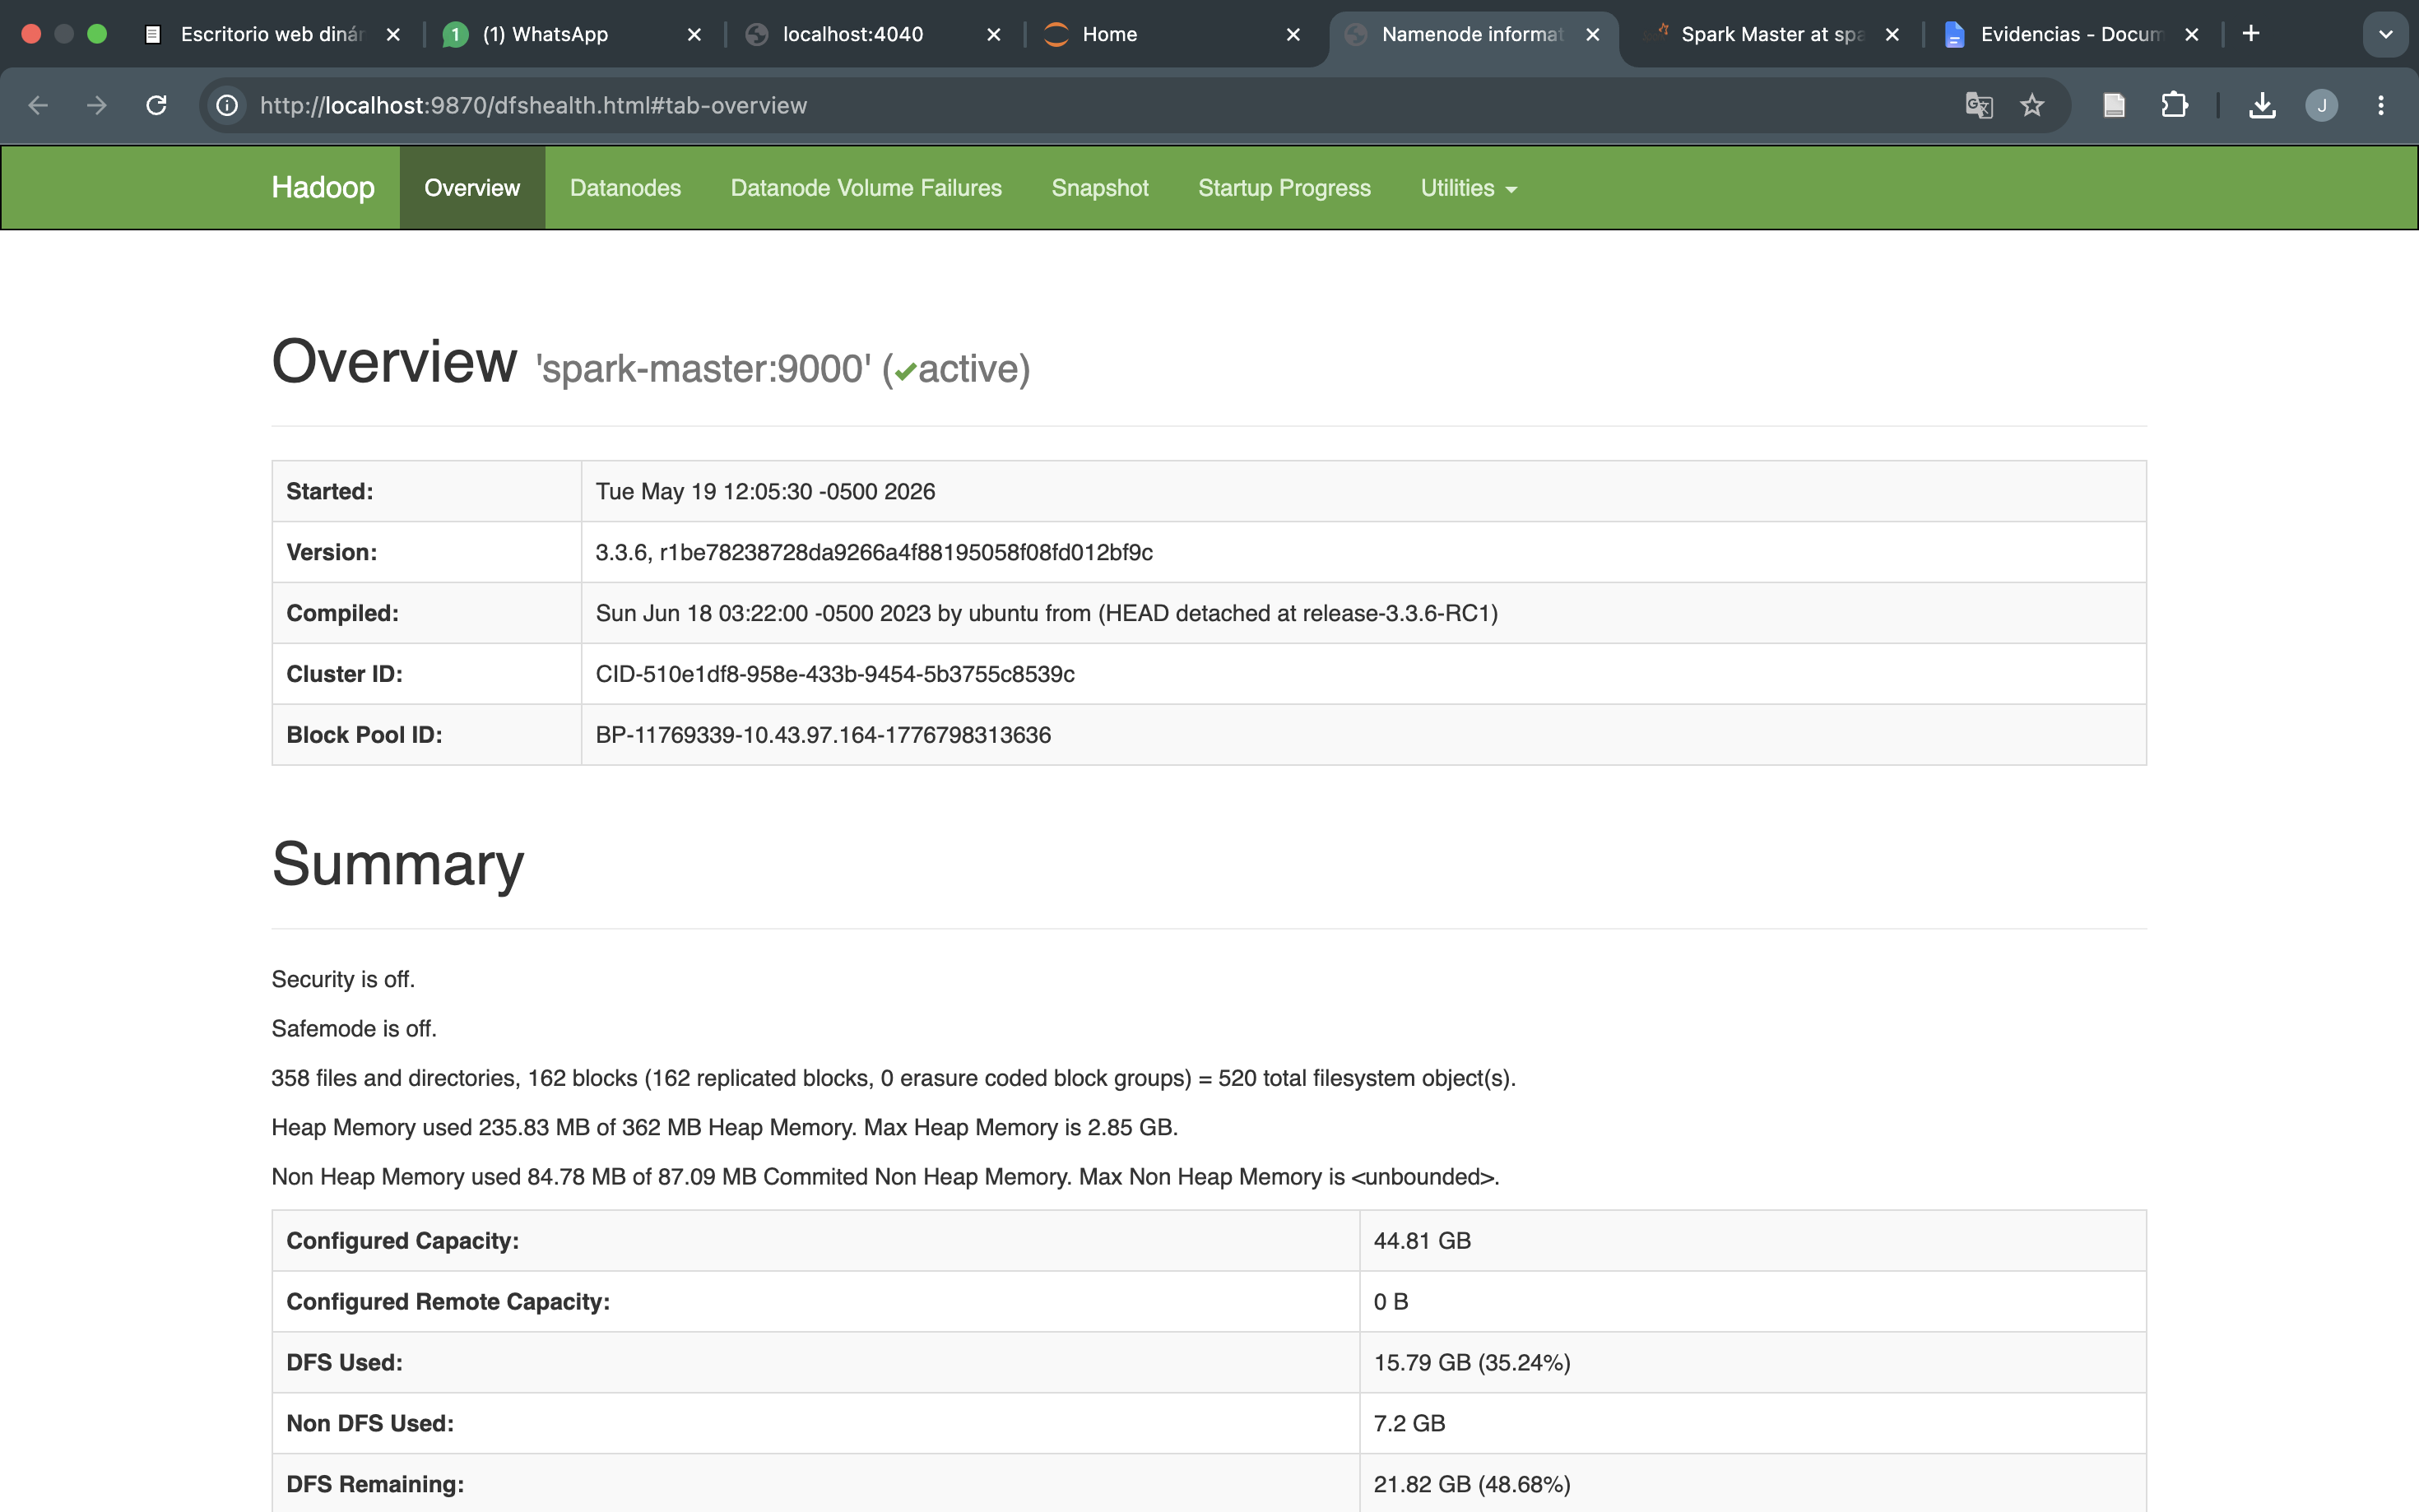
\includegraphics[width=0.95\textwidth]{figures/hdfs_overview1.png}
\caption{HDFS NameNode UI — pantalla Overview con resumen del sistema de archivos distribuido.}
\end{figure}

\begin{figure}[H]
\centering
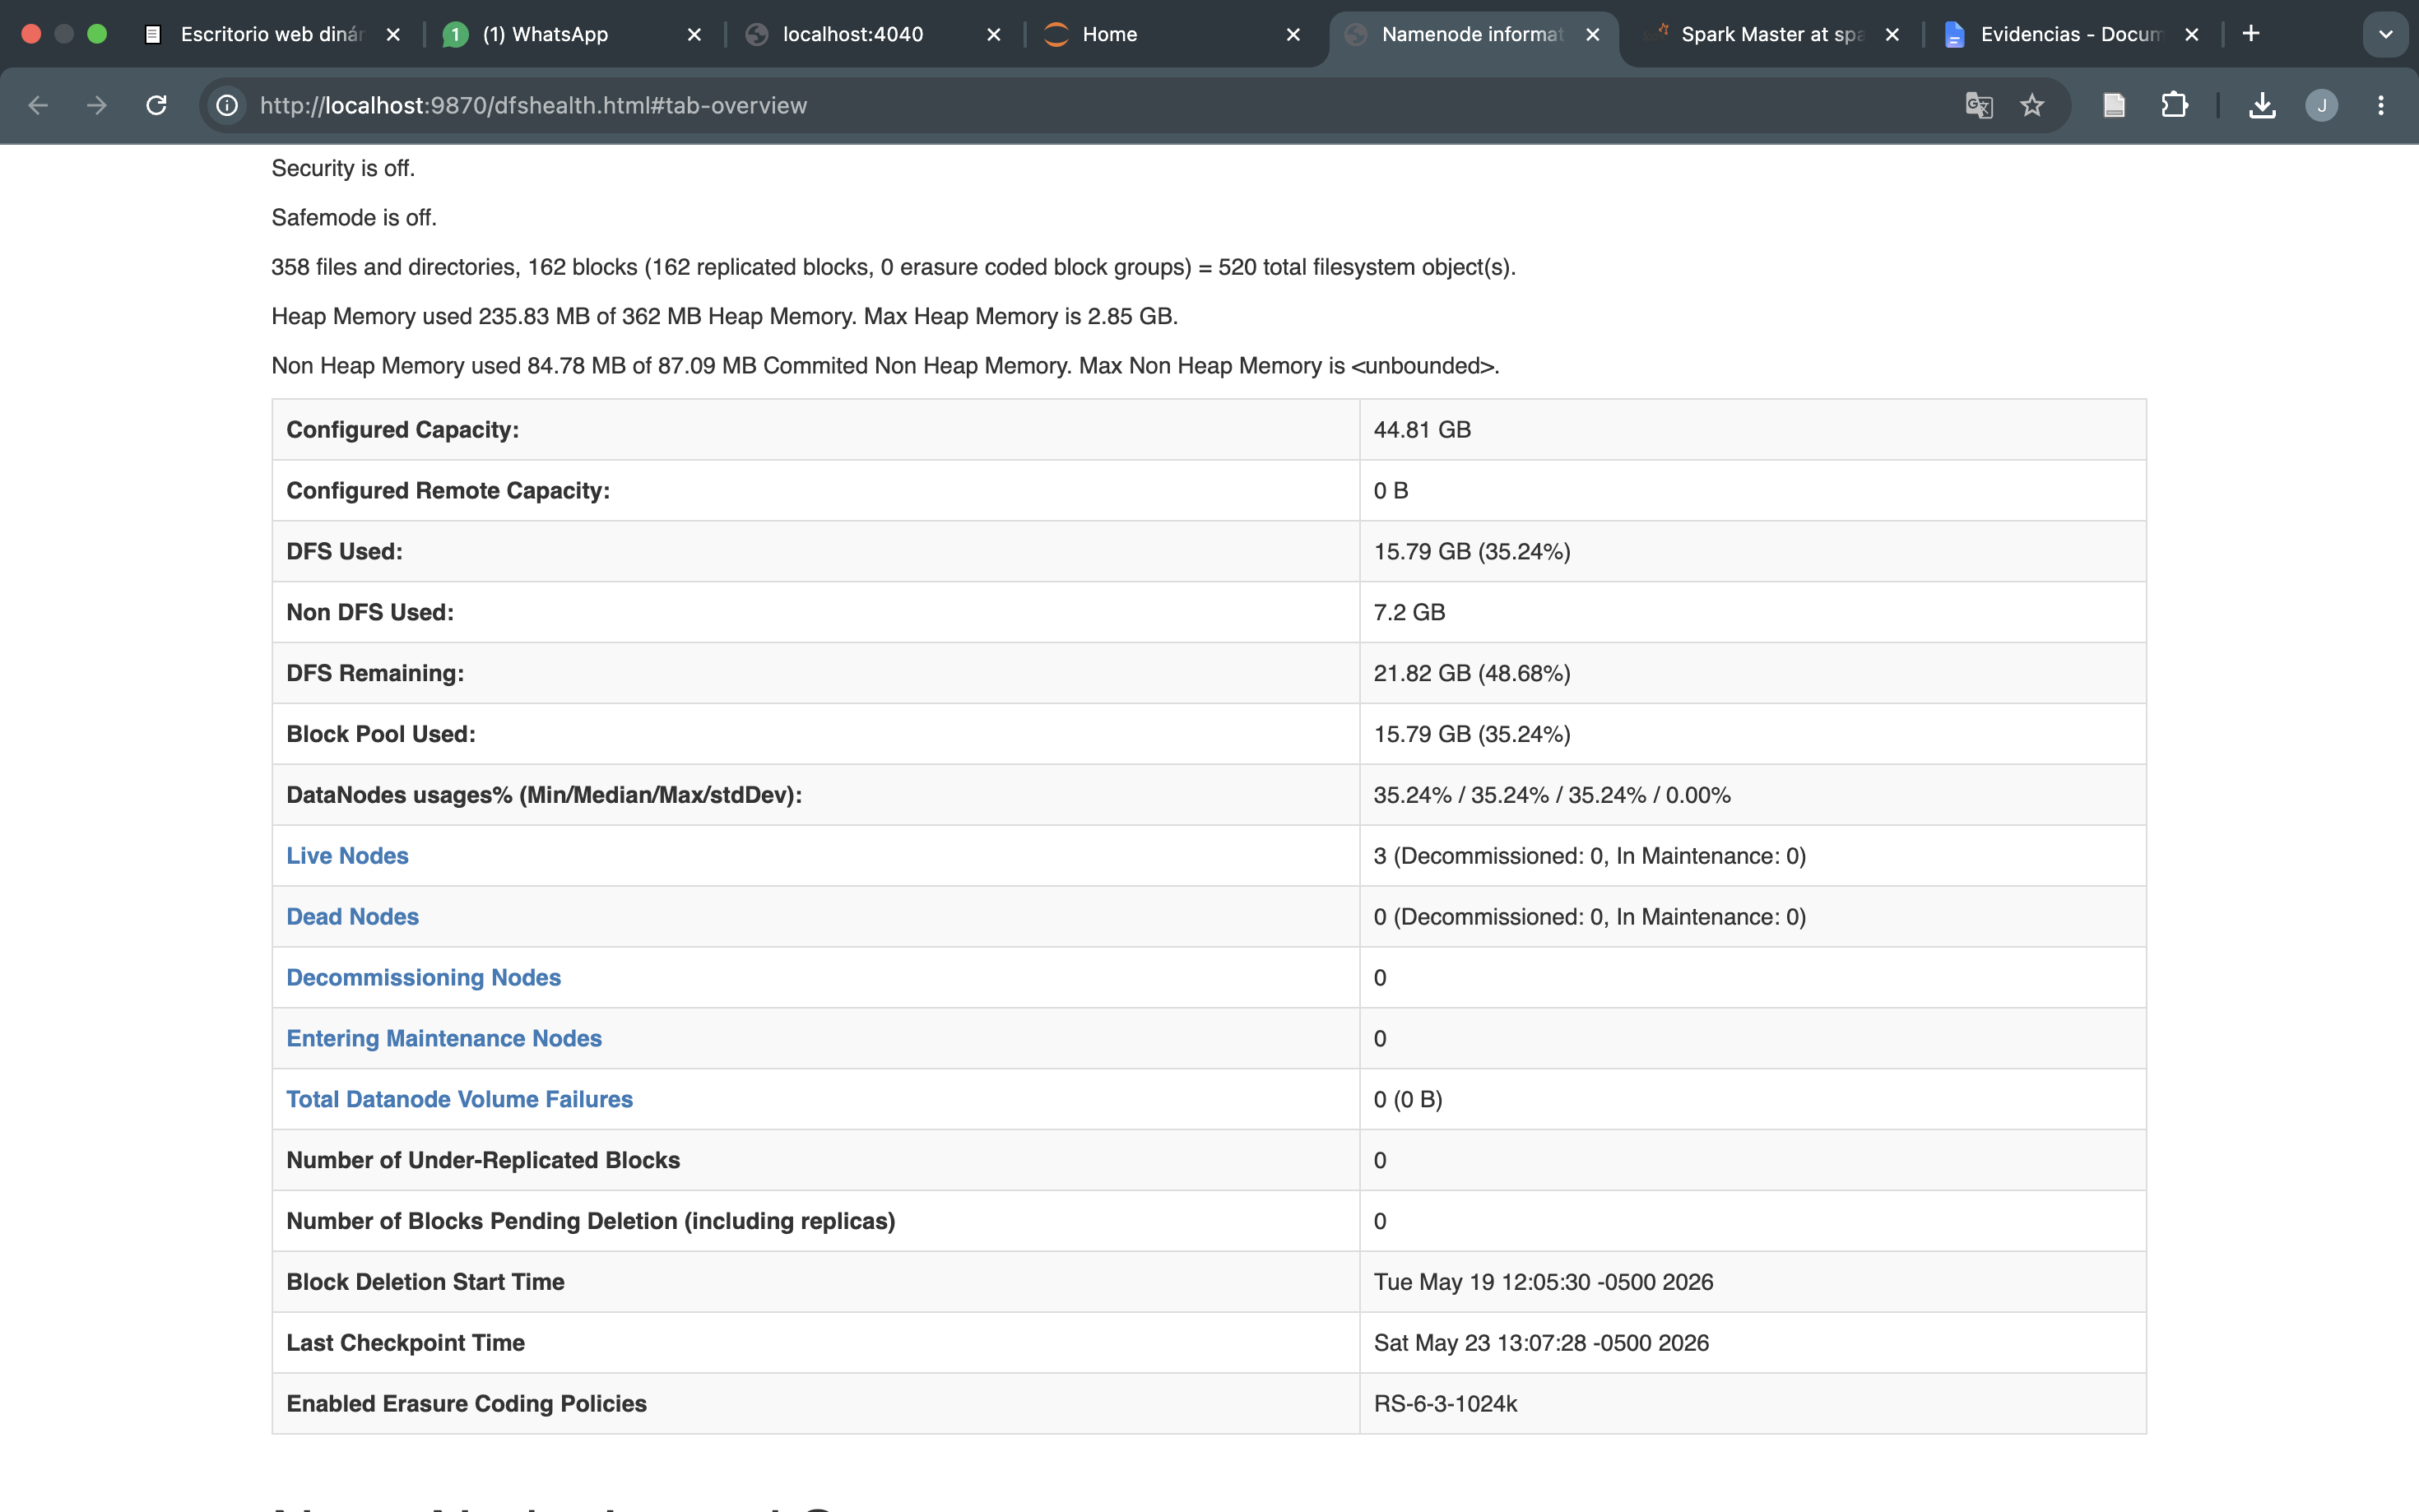
\includegraphics[width=0.95\textwidth]{figures/hdfs_overview2.png}
\caption{HDFS NameNode UI — detalles de capacidad, configuración y bloques.}
\end{figure}

\begin{figure}[H]
\centering
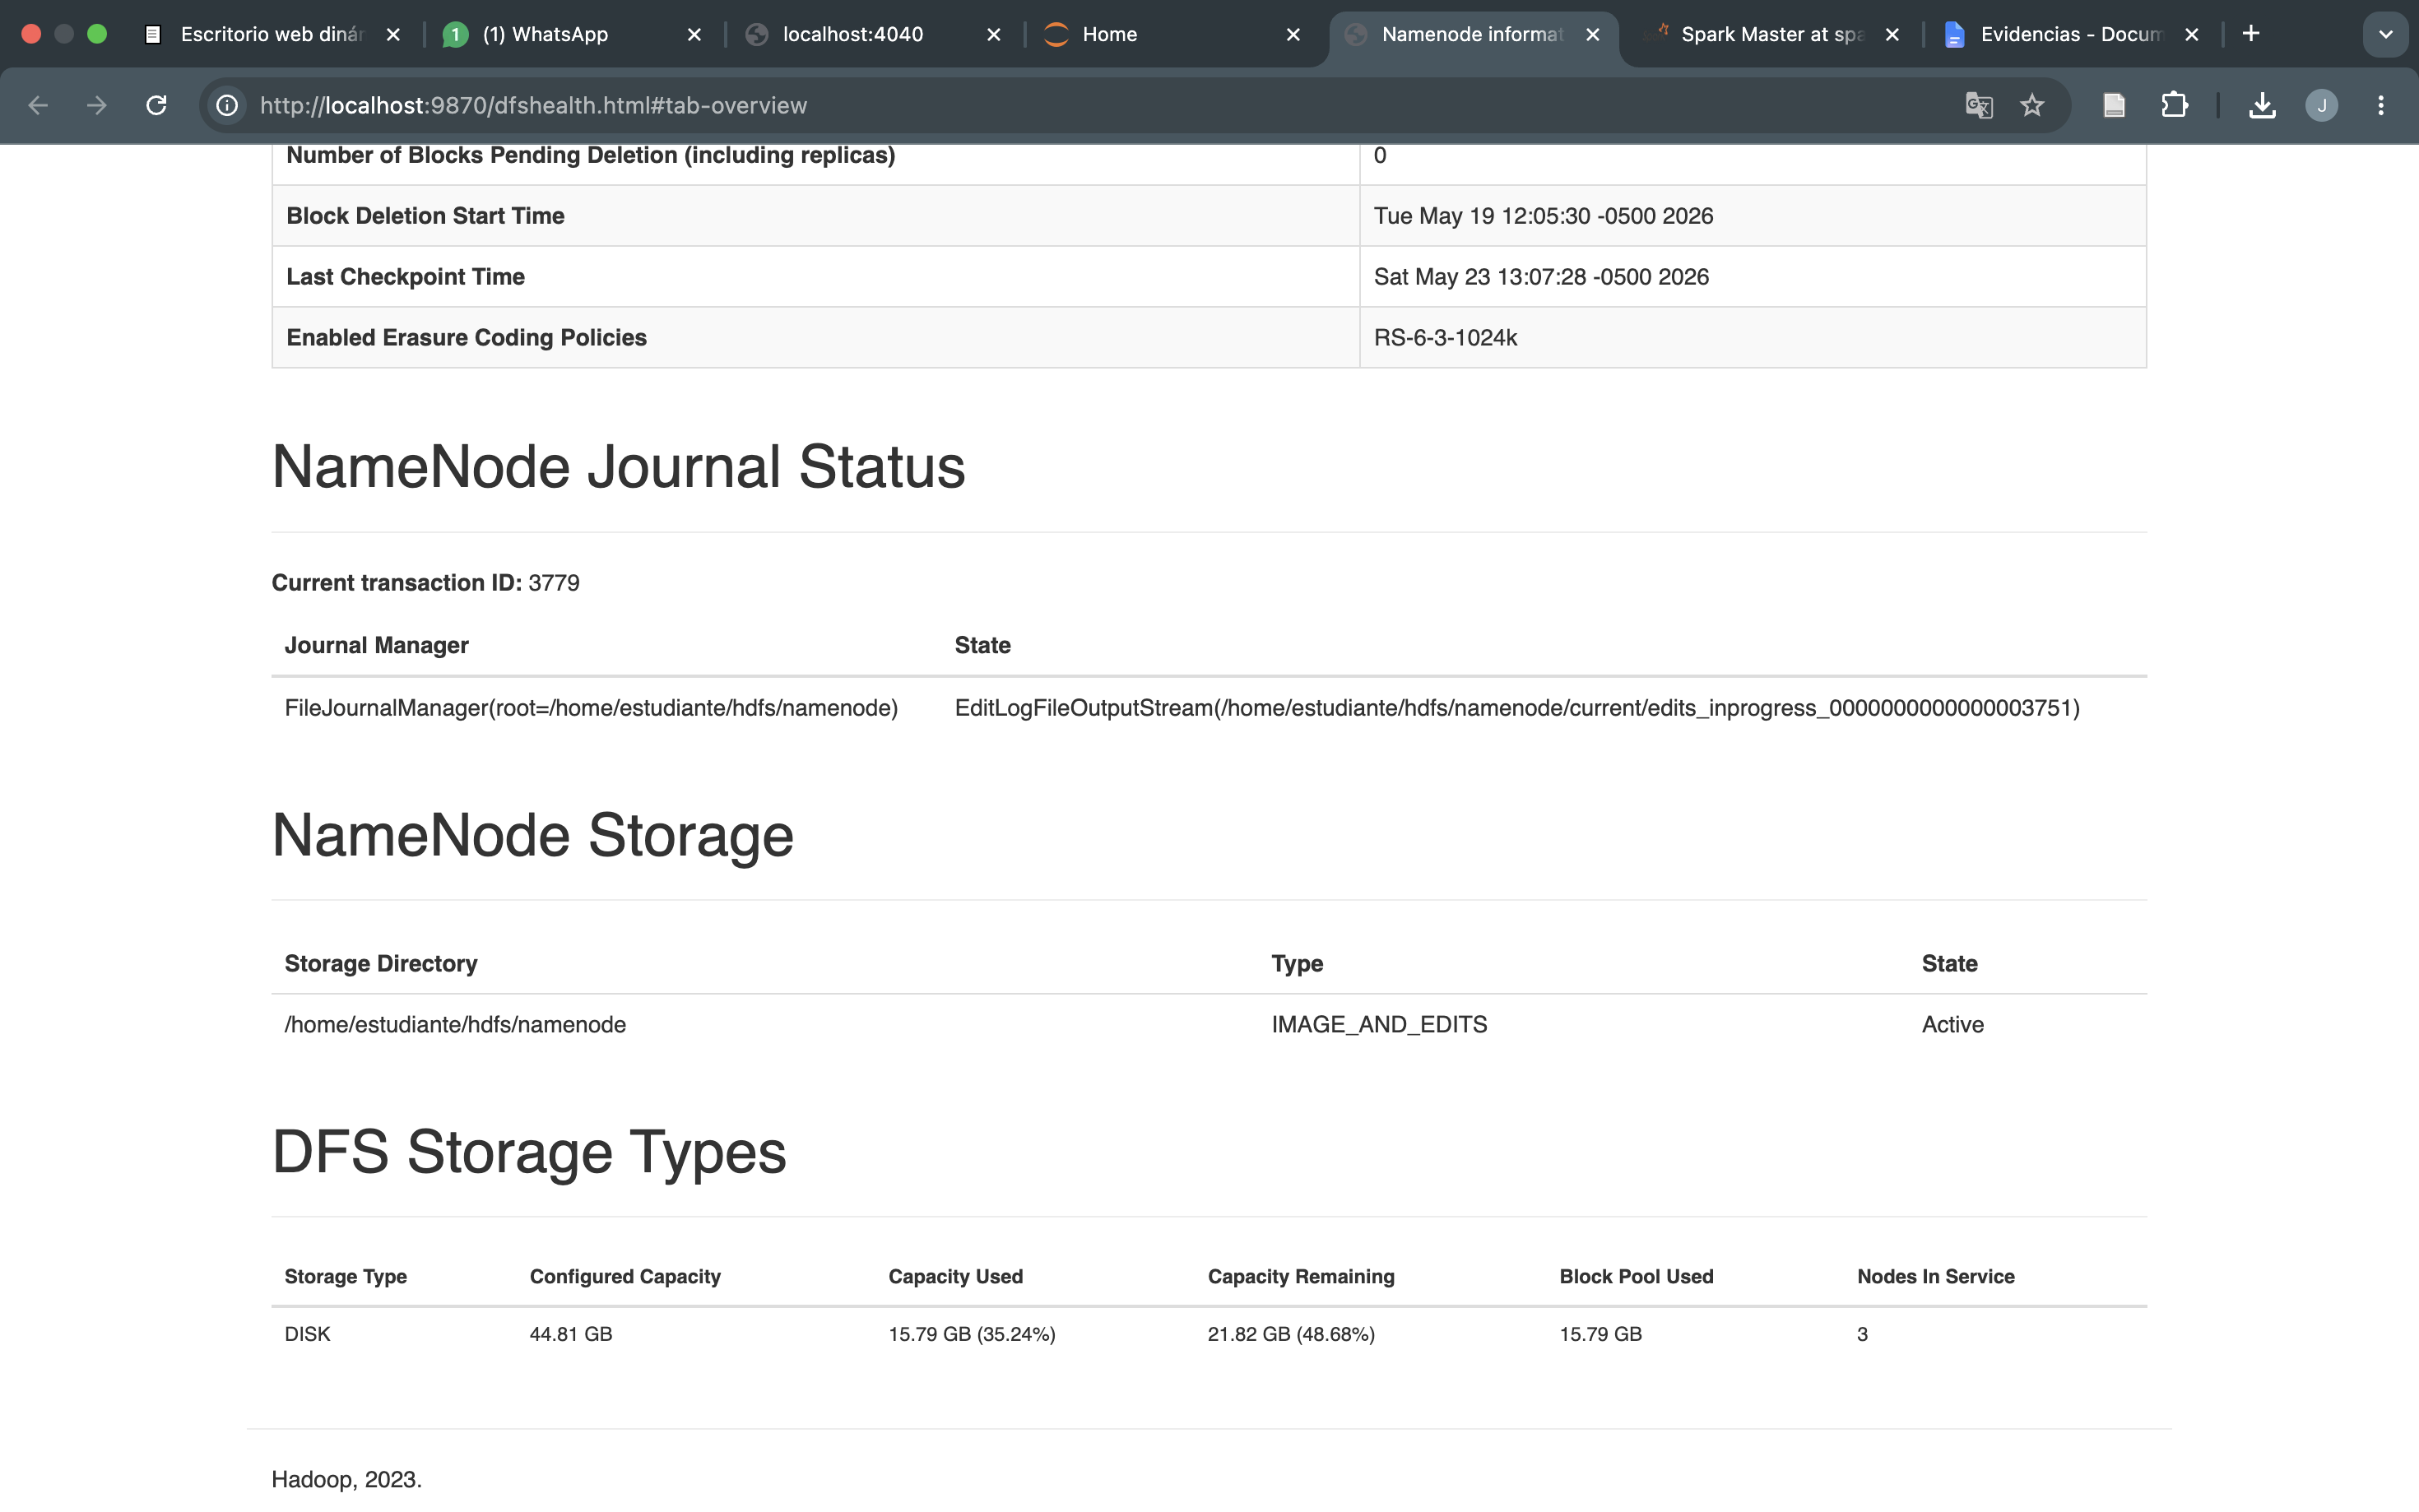
\includegraphics[width=0.95\textwidth]{figures/hdfs_overview3.png}
\caption{HDFS NameNode UI — métricas adicionales del NameNode.}
\end{figure}

\begin{figure}[H]
\centering
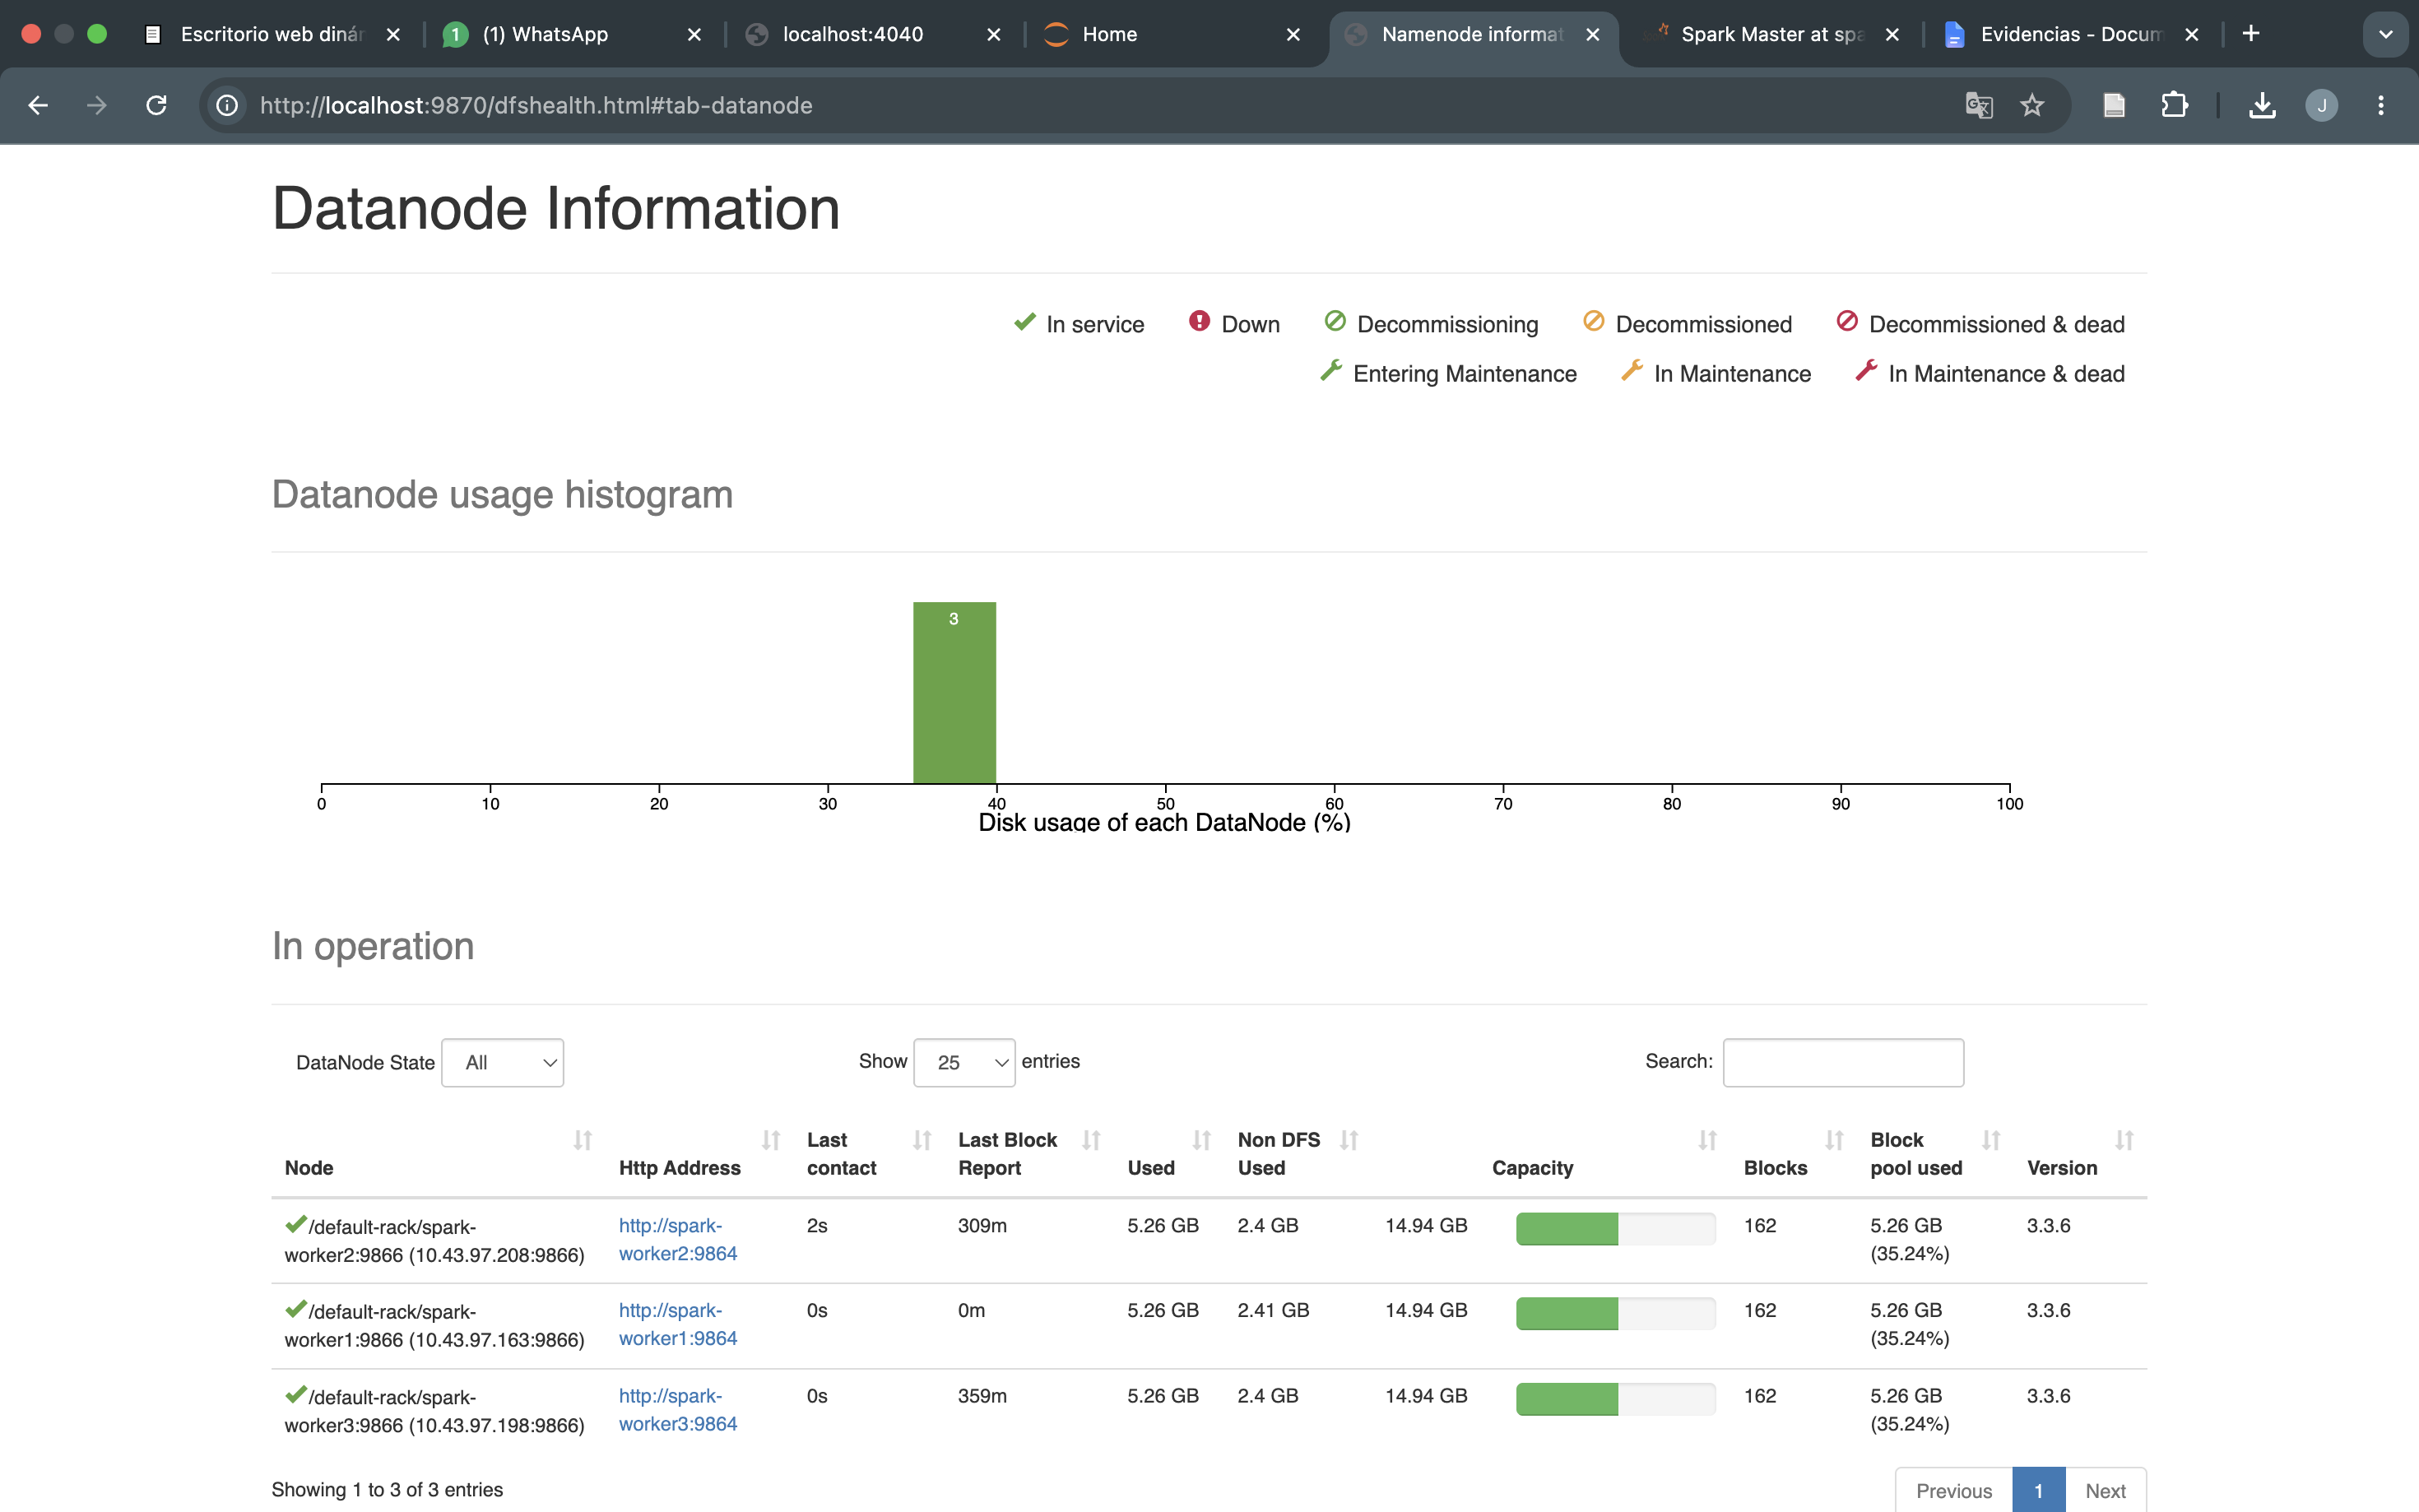
\includegraphics[width=0.95\textwidth]{figures/hdfs_datanodes.png}
\caption{HDFS NameNode UI — pestaña Datanodes mostrando los tres workers vivos con su capacidad individual.}
\end{figure}

\begin{figure}[H]
\centering
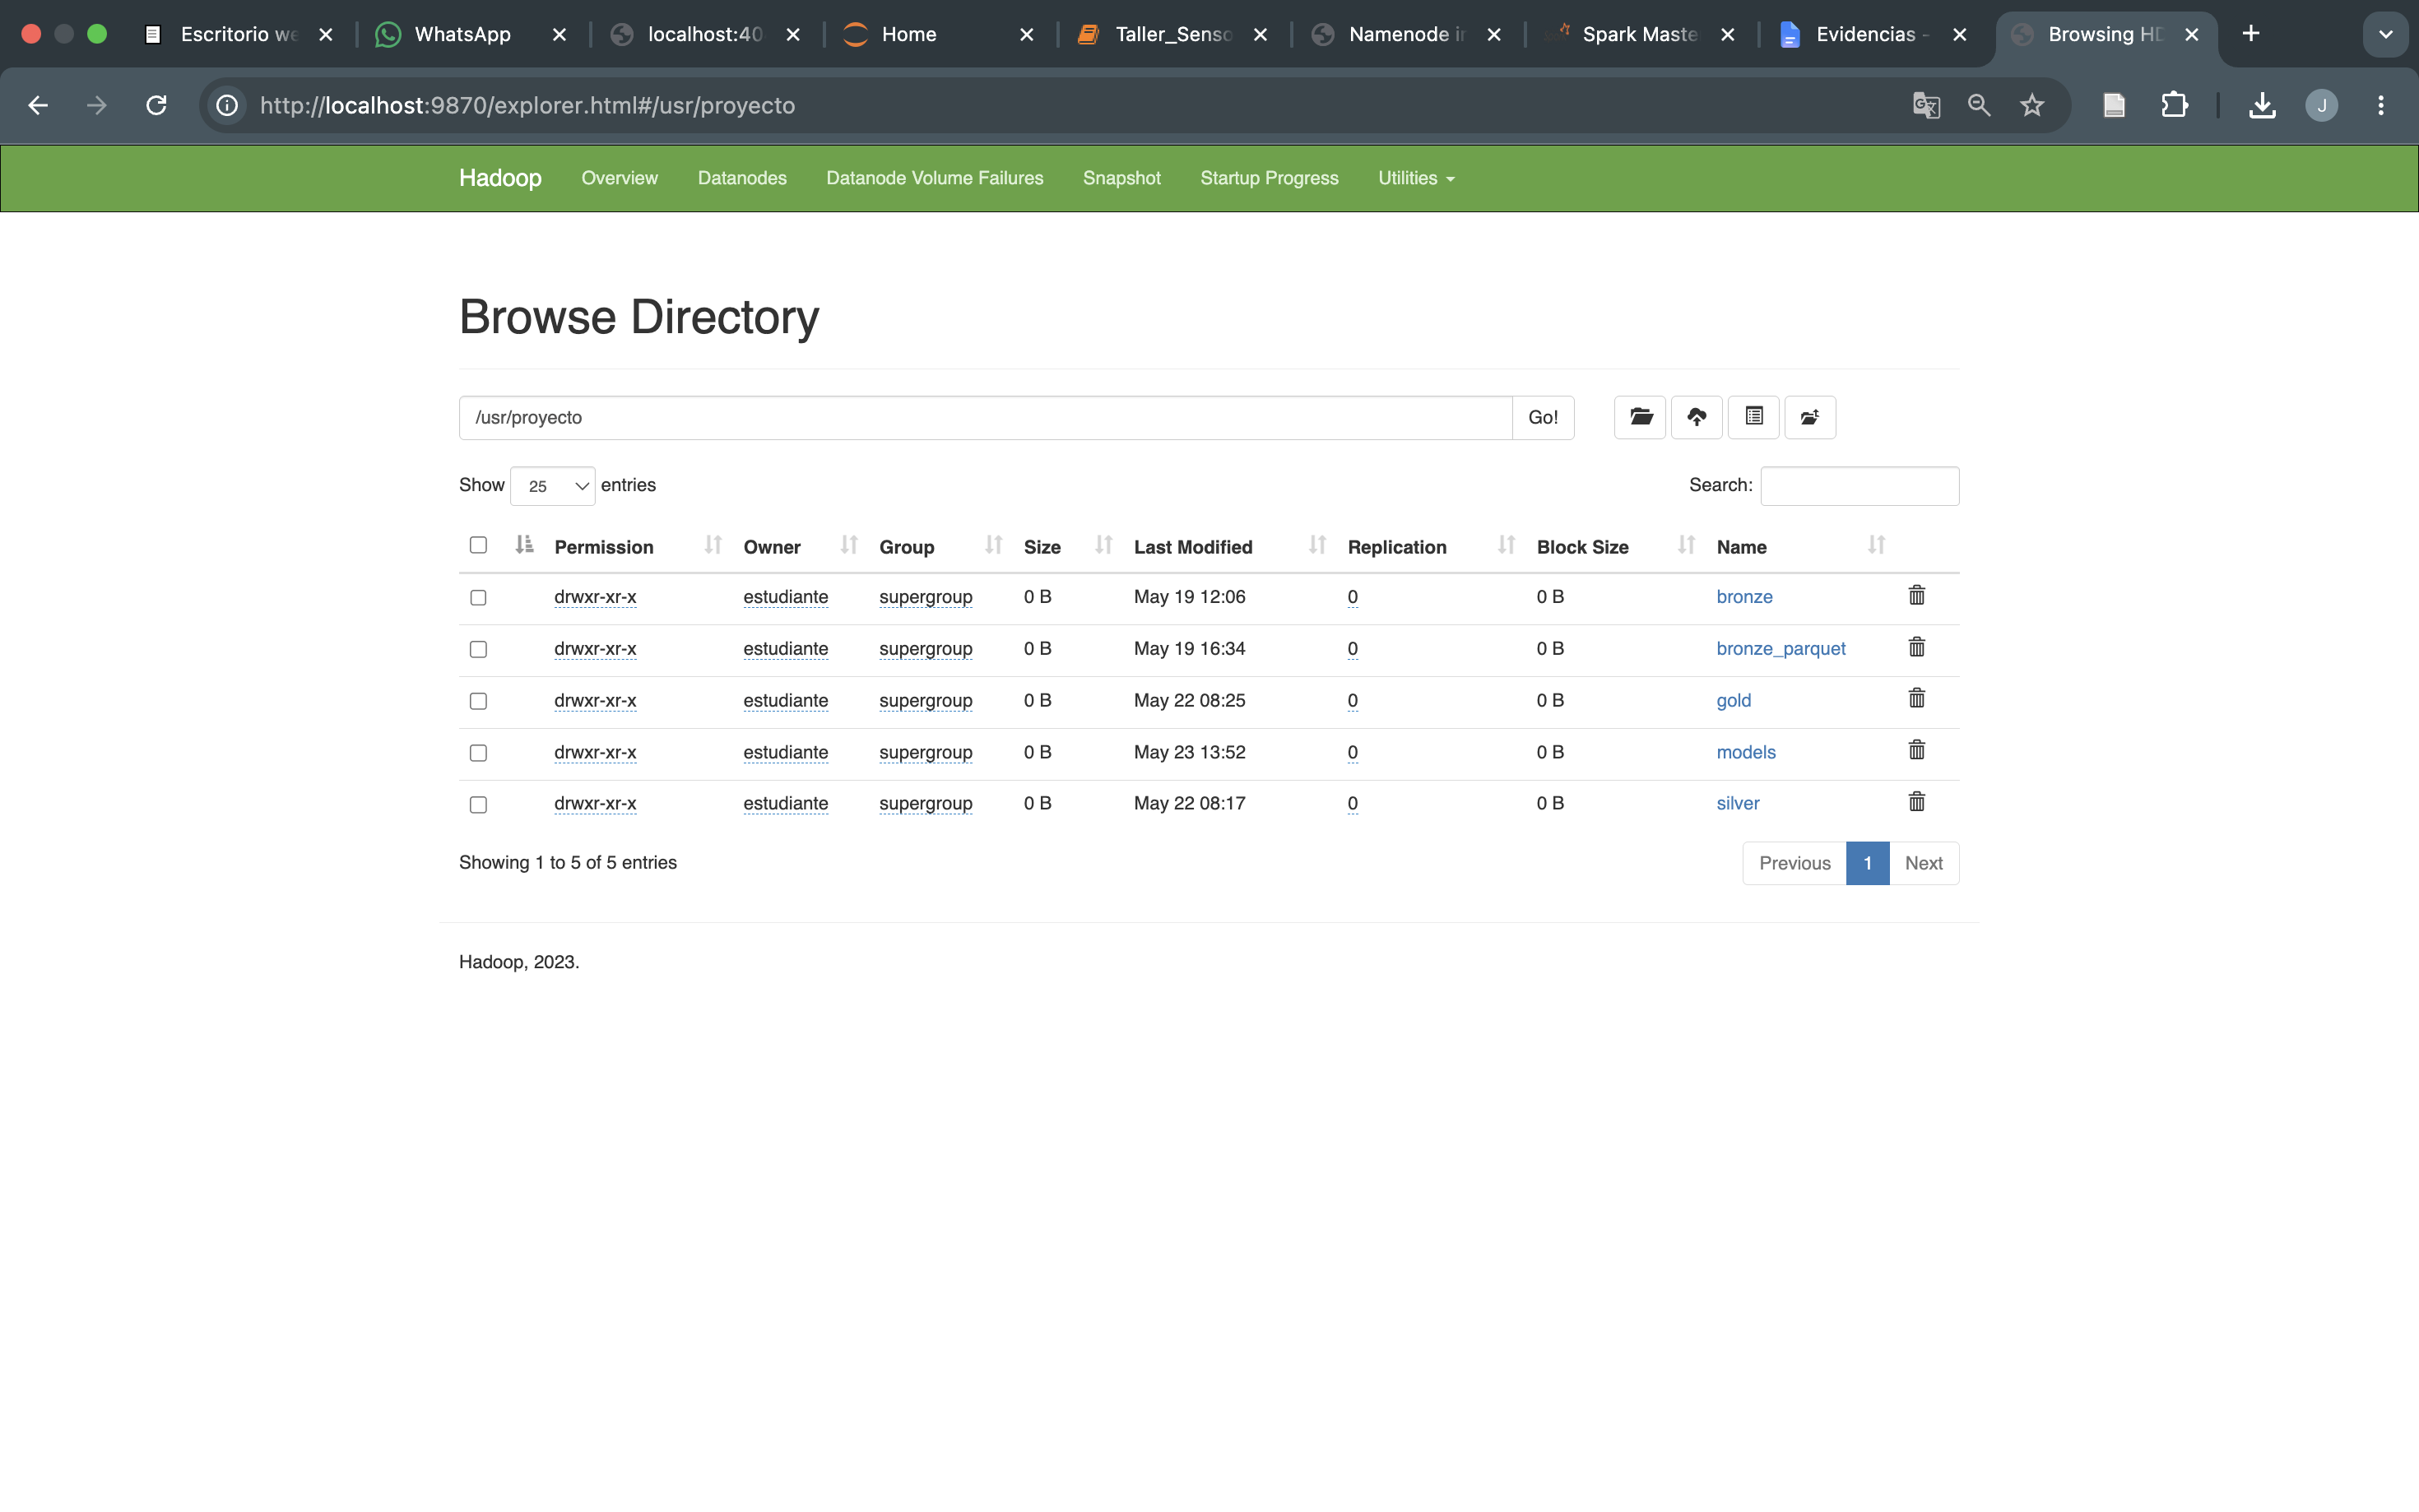
\includegraphics[width=0.95\textwidth]{figures/hdfs_browse.png}
\caption{HDFS NameNode UI — navegador del sistema de archivos sobre \texttt{/usr/proyecto/}, mostrando la estructura medallion Bronze, Silver, Gold y Models.}
\end{figure}

\subsubsection{Spark Master (puerto 8080)}
La interfaz del Spark Master expone los workers conectados, los recursos del cluster y el historial completo de aplicaciones ejecutadas durante el proyecto.

\begin{figure}[H]
\centering
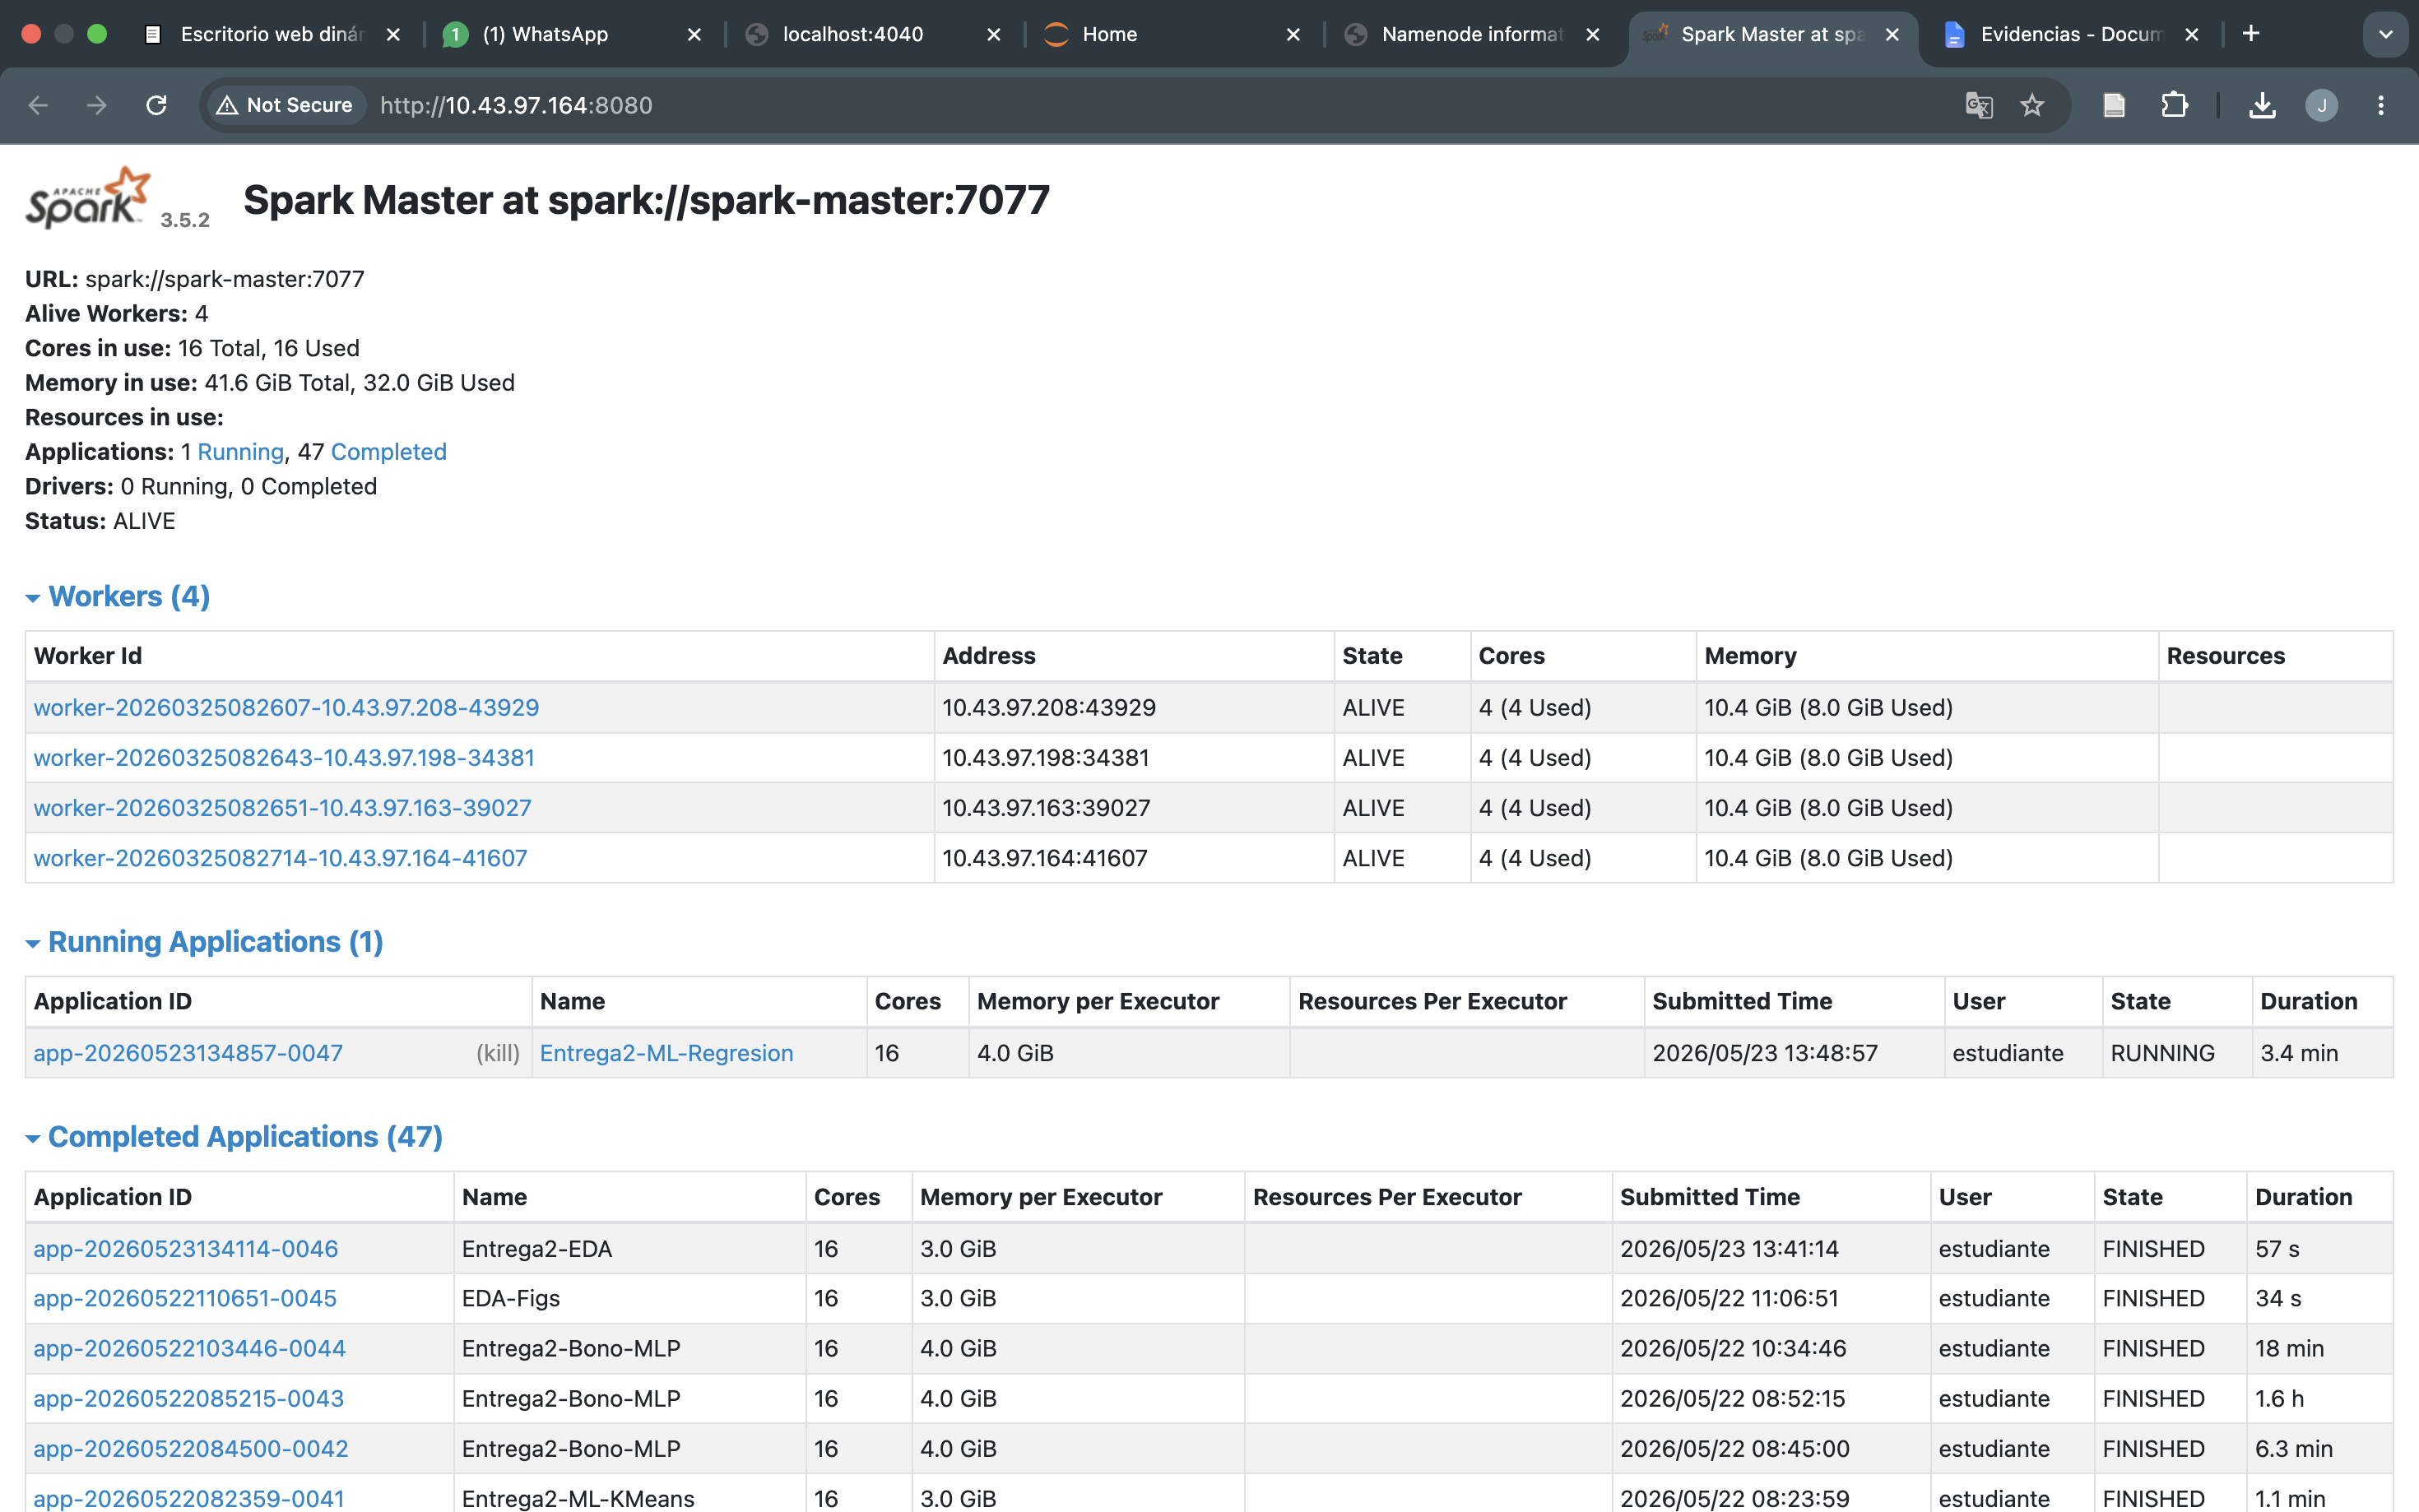
\includegraphics[width=0.95\textwidth]{figures/spark_master1.png}
\caption{Spark Master UI — workers, cores y memoria totales del cluster.}
\end{figure}

\begin{figure}[H]
\centering
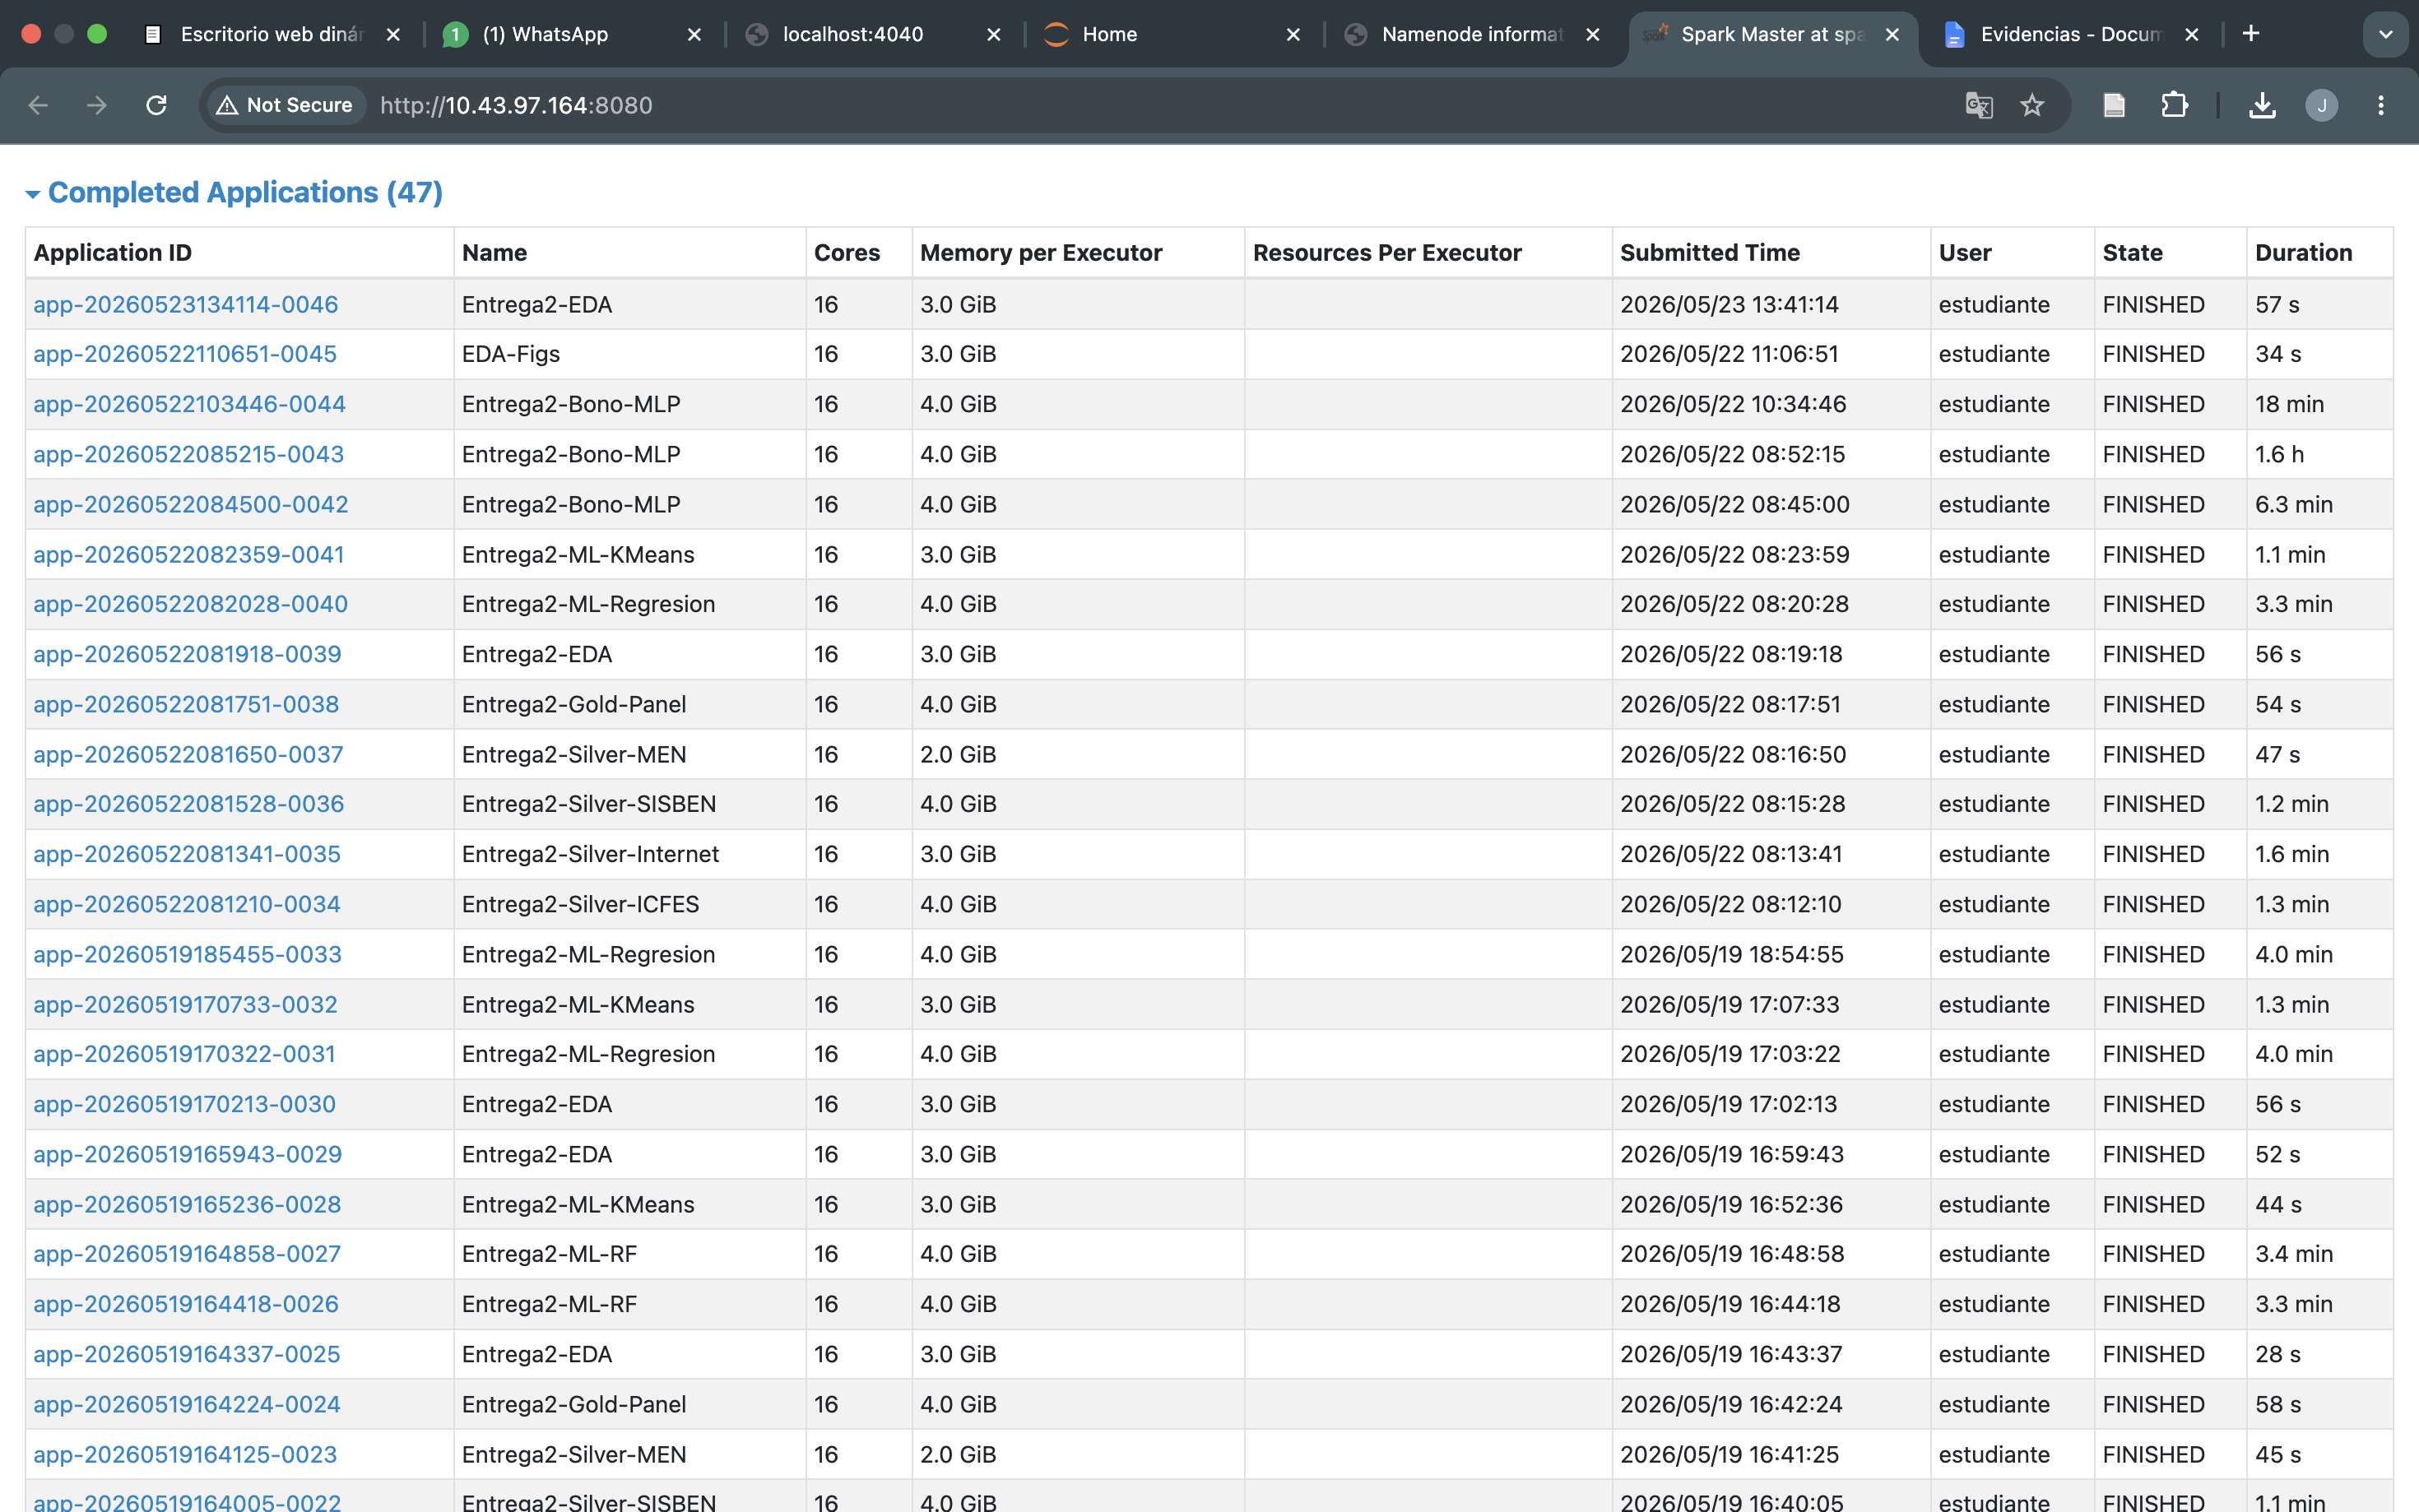
\includegraphics[width=0.95\textwidth]{figures/spark_master2.png}
\caption{Spark Master UI — historial de aplicaciones ejecutadas, incluyendo las del pipeline Bronze, Silver, Gold y los modelos de ML.}
\end{figure}

\begin{figure}[H]
\centering
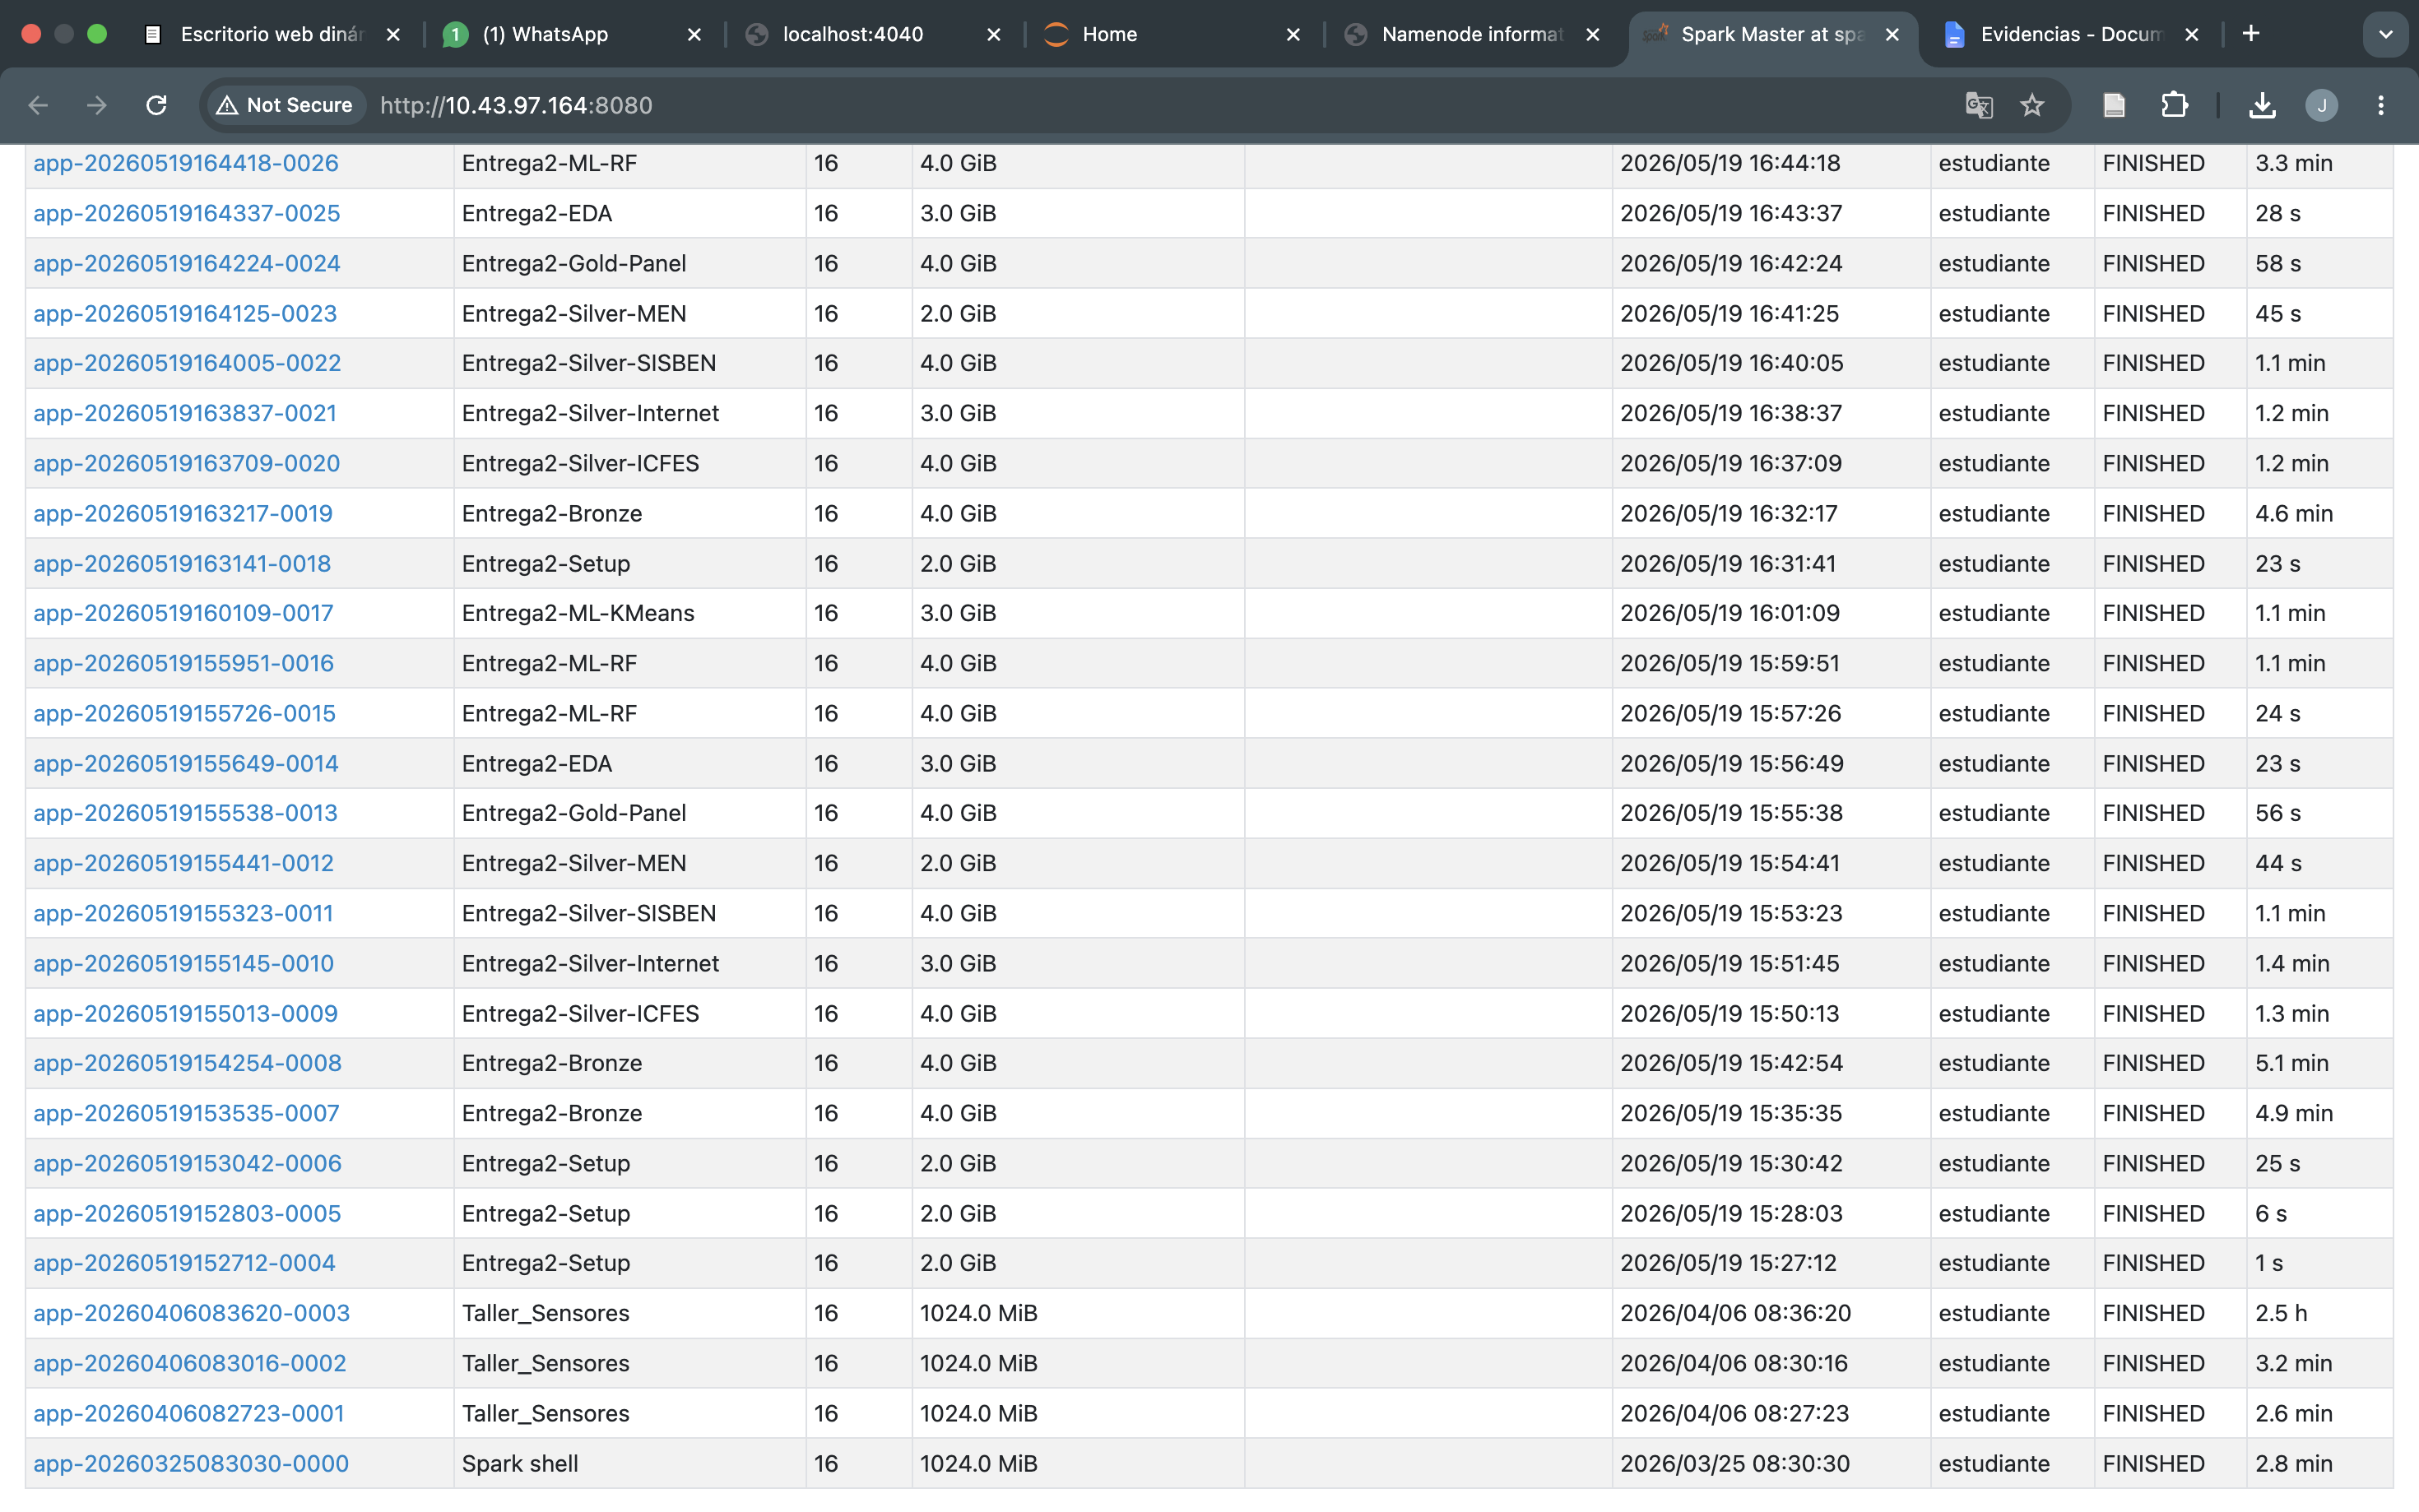
\includegraphics[width=0.95\textwidth]{figures/spark_master3.png}
\caption{Spark Master UI — detalle adicional del historial de aplicaciones.}
\end{figure}

\subsubsection{Spark Application UI (puerto 4040)}
La interfaz de aplicación de Spark detalla la ejecución distribuida de una aplicación específica, mostrando jobs, stages y los executors asignados sobre los workers.

\begin{figure}[H]
\centering
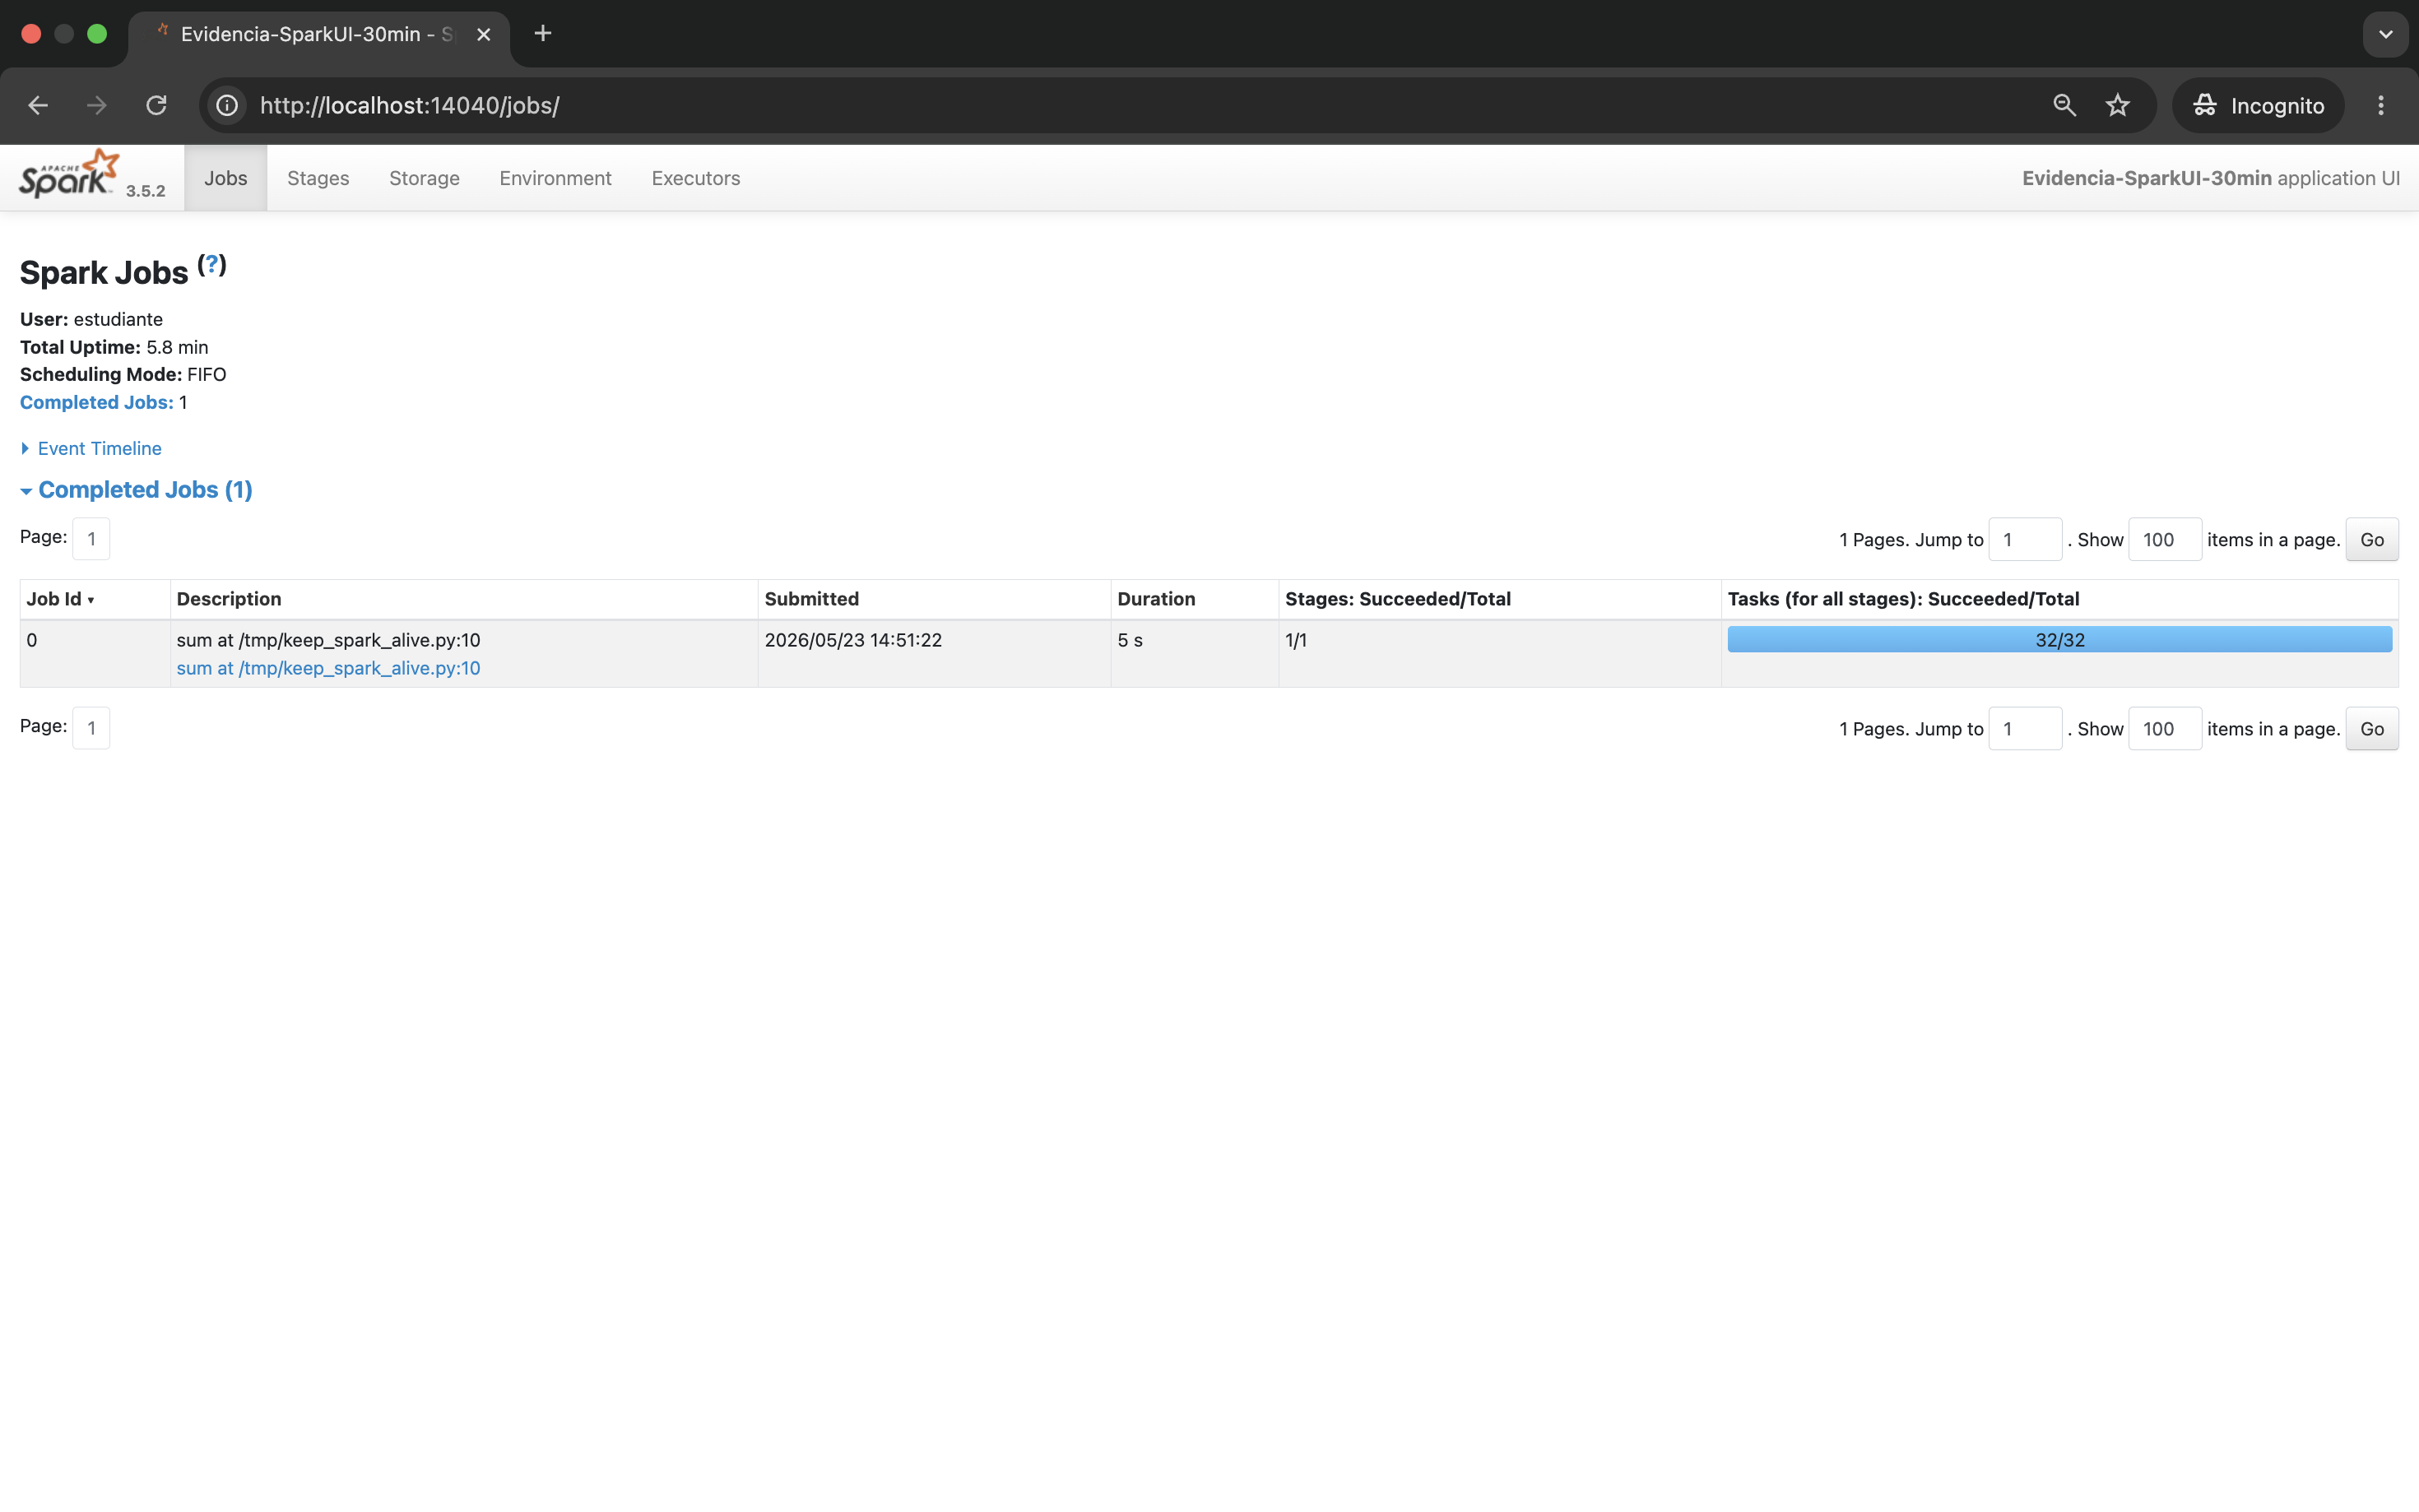
\includegraphics[width=0.95\textwidth]{figures/spark_jobs.png}
\caption{Spark Application UI — pestaña Jobs con la lista de operaciones disparadas por la aplicación y su duración.}
\end{figure}

\begin{figure}[H]
\centering
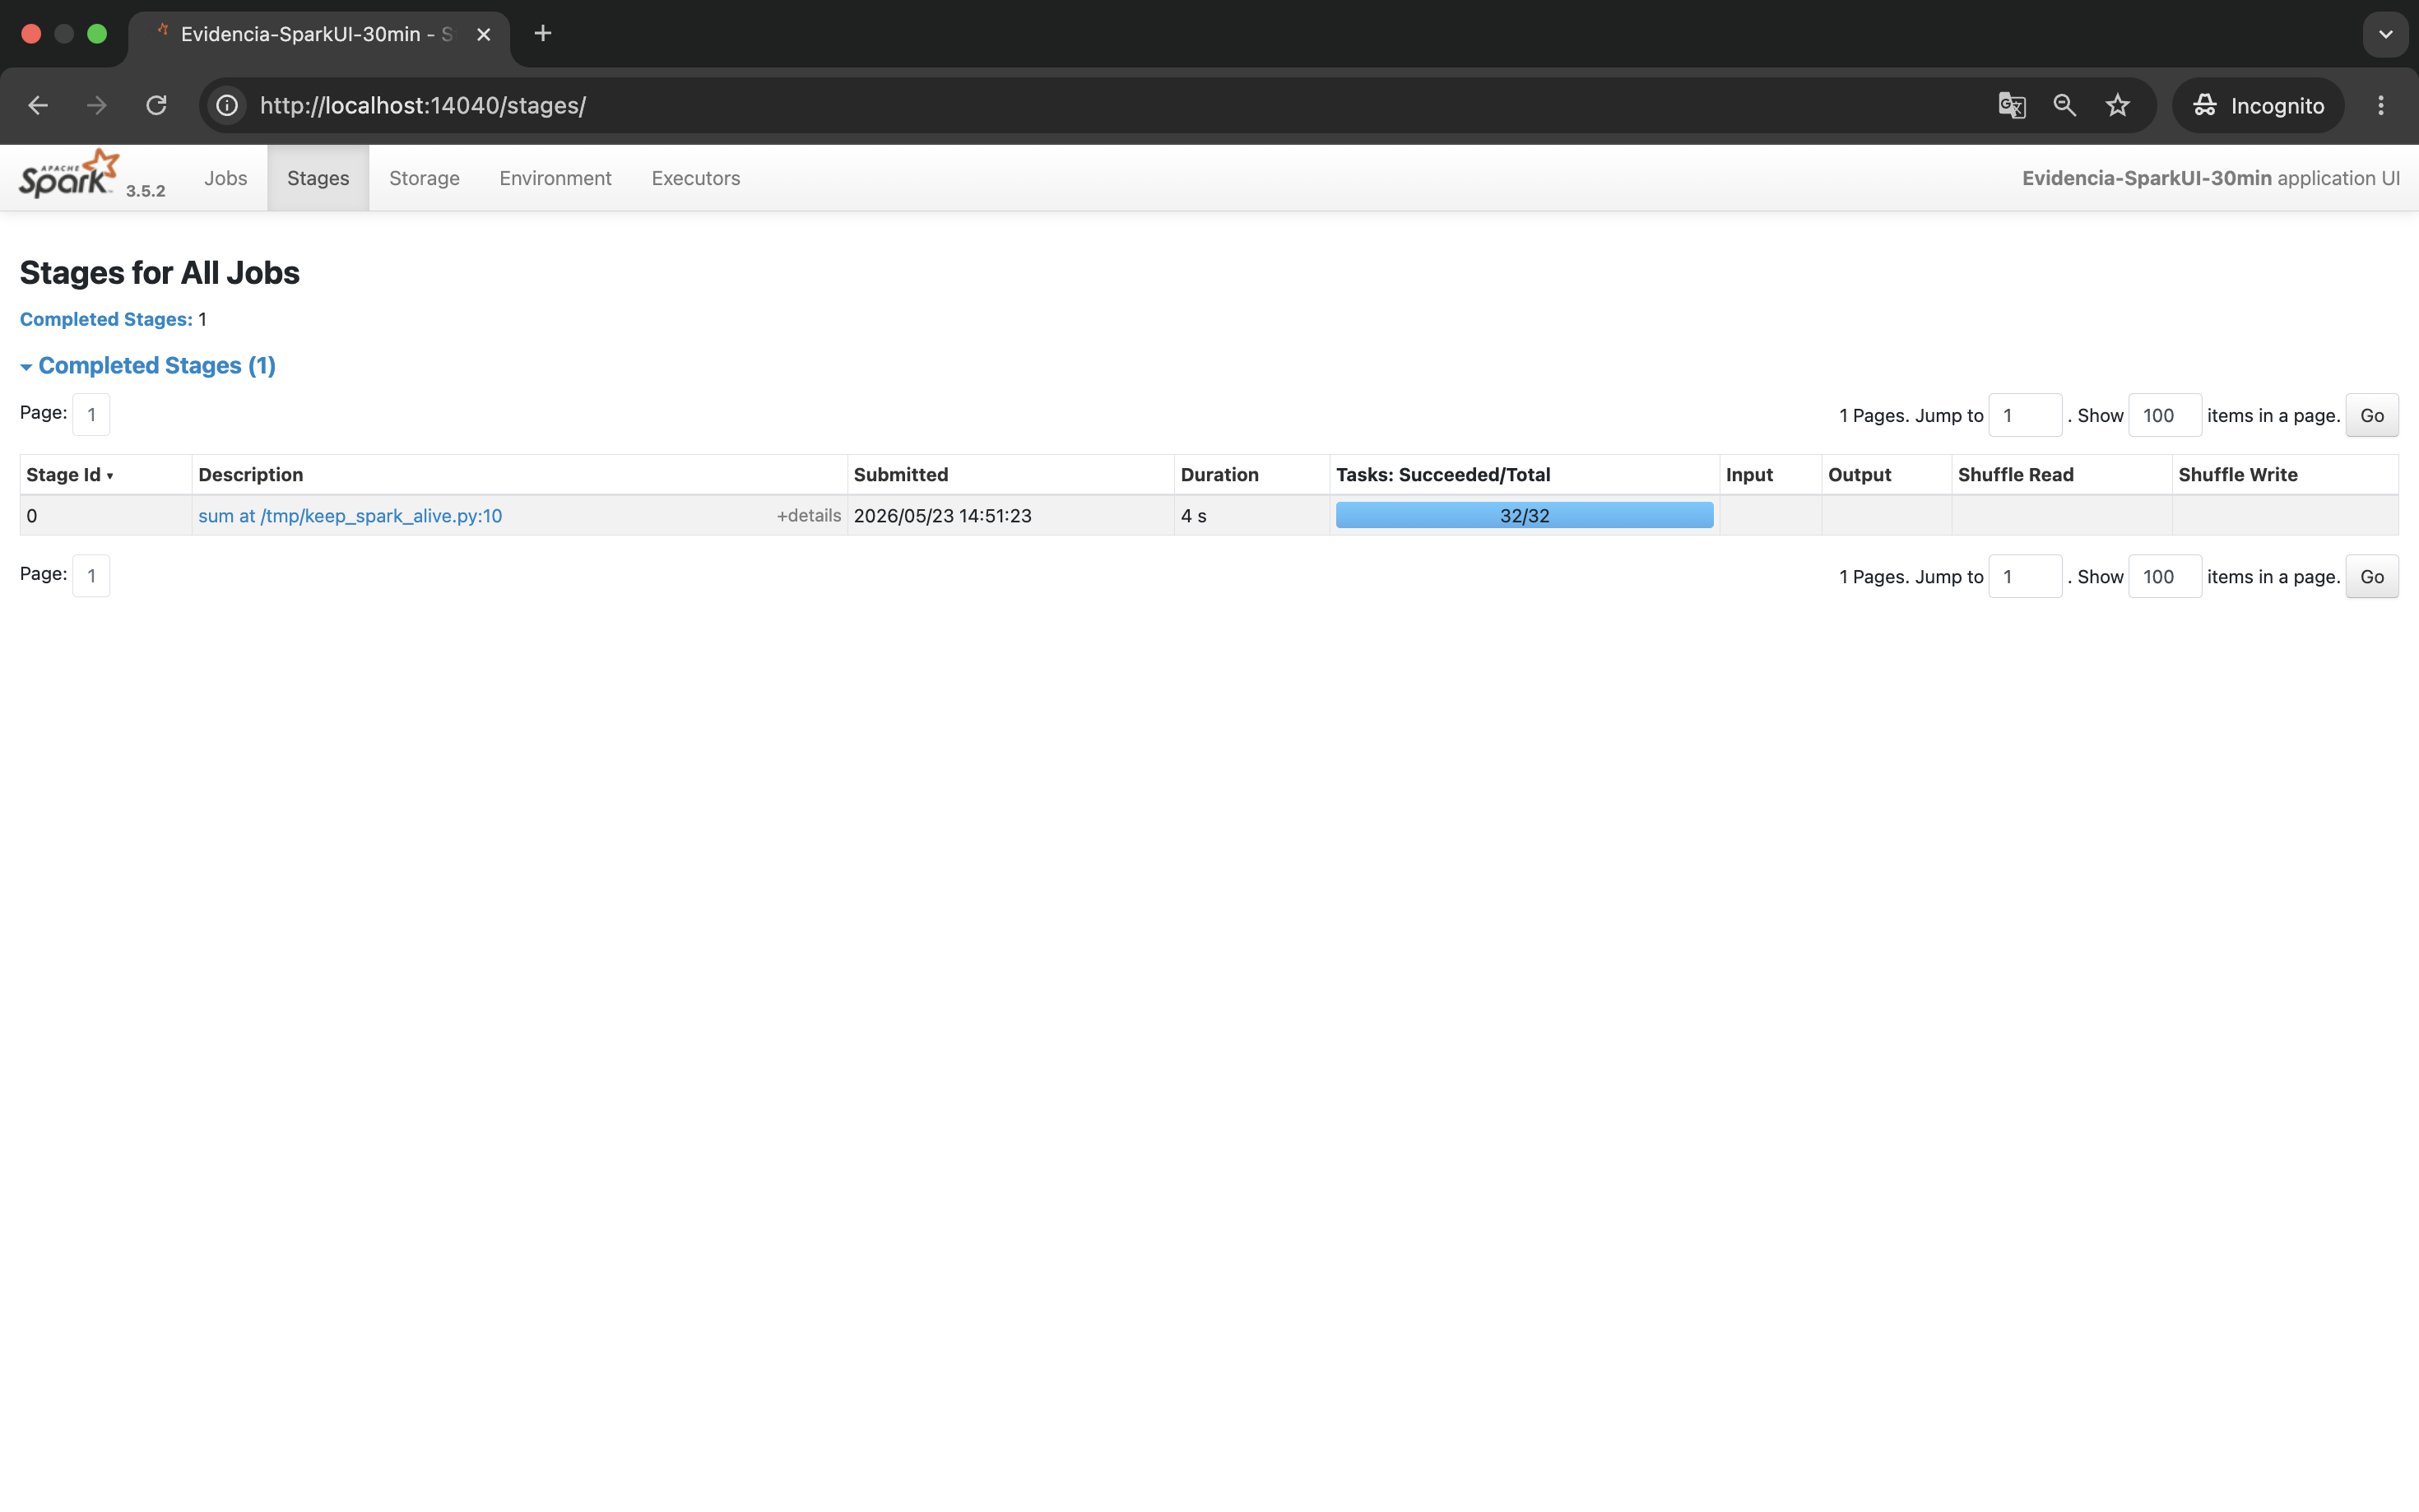
\includegraphics[width=0.95\textwidth]{figures/spark_stages.png}
\caption{Spark Application UI — pestaña Stages mostrando la descomposición de los jobs en stages paralelos y el progreso de cada uno.}
\end{figure}

\begin{figure}[H]
\centering
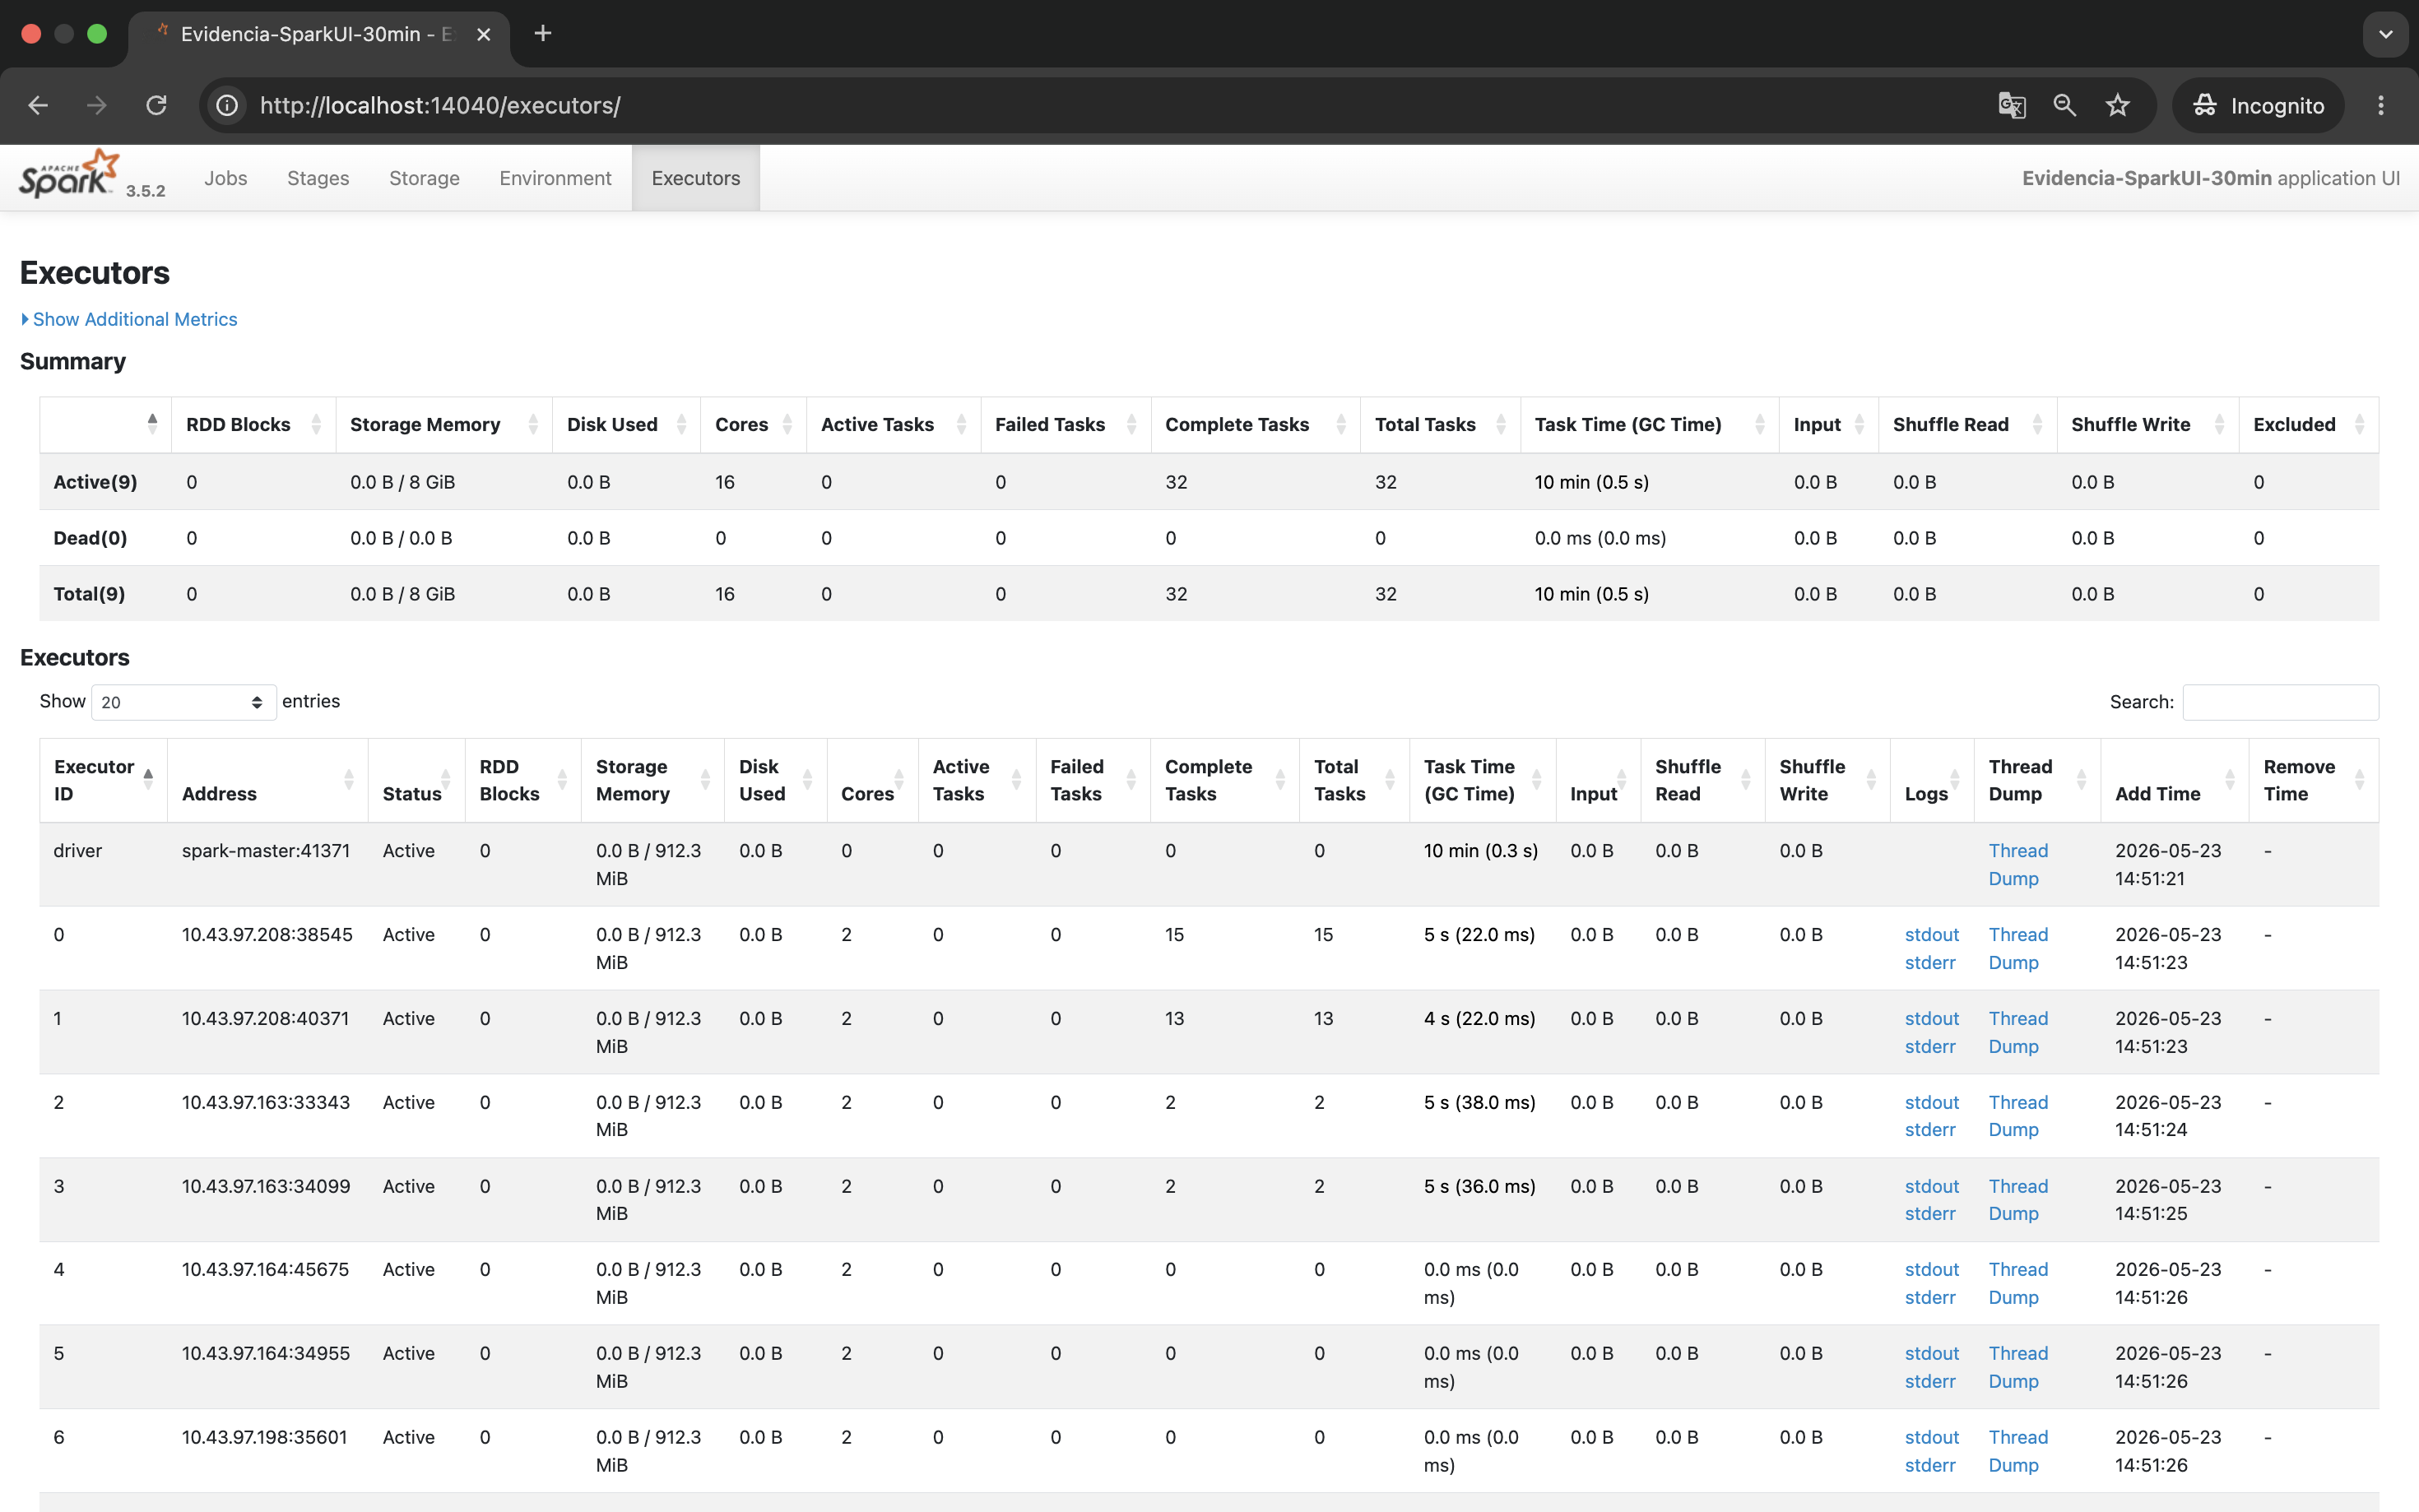
\includegraphics[width=0.95\textwidth]{figures/spark_executors.png}
\caption{Spark Application UI — pestaña Executors evidenciando los workers reales del cluster asignados a la aplicación (driver más executors distribuidos).}
\end{figure}

Estas capturas confirman que el pipeline no se limita a una ejecución local: se distribuye sobre los cuatro workers del cluster, aprovechando los 16 cores y 42 GB de RAM disponibles, y persiste tanto datos como modelos sobre HDFS con replicación 3.
